\documentclass[12pt,a4paper]{report}

%###################################################################################
%###################### Document Defintions ########################################
%###################################################################################
%aubrey: no real need to change these
%how to handle spaces
\sloppy
\makeindex

\usepackage[utf8]{inputenc} %changed document encoding before to UTF8
\usepackage[UKenglish]{babel}

\usepackage{amsmath, marvosym} % Mathematik
%\usepackage{harvard} %for harvard style citation, keep this position before url package
\usepackage{cite} %added by MM
%\usepackage{natbib} %bibliography from BADS
%\usepackage{bibgerm}

\usepackage{times, url, geometry, amssymb, booktabs, html}
\usepackage{hyperref} %Hyperlinks zw. Textstellen
\usepackage[pdftex]{graphicx} %pdf figures
\usepackage{subfig} %multi-figures
\usepackage{listings} %code listings
\usepackage{multirow} %for multi-row tables
\usepackage{color} %needed for listings
%\usepackage{todonotes} %for annotations
\usepackage[show]{chato-notes} %note/todo/inote/citeMissing - change to [hide]
\usepackage{qtree}

%depth of section
\setcounter{secnumdepth}{4}
%depth of TOC
\setcounter{tocdepth}{3} 
%directory for graphics
\graphicspath{{gfx/}}

%setting for listing
\lstset{
	extendedchars=true,
	basicstyle=\scriptsize\ttfamily,
	%basicstyle=\tiny\ttfamily,
	tabsize=2,
	keywordstyle=\textbf,
	commentstyle=\color{grau},
	stringstyle=\textit,
	numbers=left,
	numberstyle=\tiny,
	% für schönen Zeilenumbruch
	breakautoindent  = true,
	breakindent      = 2em,
	breaklines       = true,
	postbreak        = ,
	%prebreak         = \raisebox{-.8ex}[0ex][0ex]{\ensuremath{\lrcorner}},
	prebreak         = \raisebox{-.8ex}[0ex][0ex]{\Righttorque},
}

%Table of Content TOC settings
\setcounter{tocdepth}{3}
%This is needed for entering URLs for harvard citation style
%\renewcommand{\harvardurl}{URL: \url}


%###################################################################################
%########################### Thesis content ########################################
%###################################################################################
\begin{document}
%__________________________Start_of_Thesis______________________________________________
%Roman numeral numbering for initial section of thesis
\pagenumbering{roman}
%title page specification, deployed as seperate file the input folder
%############################################################################
%########################### Change This ####################################
%############################################################################
%alt title: Survey of ...
\newcommand{\trtitle}{Development and Evaluation of a Service Bot for the e-Government Sector}
\newcommand{\trtype}{Bachelor Thesis}
\newcommand{\trauthor}{Mohamed Megahed}
\newcommand{\trmatrikelnummer}{342655}
%supevisor
\newcommand{\trbetreuerA}{Dr. Andreas Lommatzsch}
%estimator 1
\newcommand{\trguta}{Prof. Dr. Dr. h.c. \c{S}ahin Albayrak}
%estimator two
\newcommand{\trgutb}{Prof. Dr. Odej Kao}
\newcommand{\trdate}{\today}

%############################################################################
%########################### DO NOT touch this, unless you need to ##########
%############################################################################
\thispagestyle{empty}
%head line logo + tub + logo
\begin{tabular}{lcc}
\includegraphics[width=0.15\textwidth]{template/TUBerlin_Logo_rot_hell}& \hspace{1.1cm} Technische Universit{\"a}t Berlin& \hspace{1.2cm} 
\includegraphics[width=0.15\textwidth]{template/aot_logo}\\
\end{tabular}
%draw a line
\rule{\textwidth}{0.4pt}
%aub: remove this on final submission
\begin{center}
DOCUMENT BUILD DATE: \today\\%
%add your status here, e.g. First Draft for Supervisor etc.
DOCUMENT STATUS: Semi-Final Draft (Impl., Eval. Concl.)
\end{center}

%vertical space
\vspace{2.5cm}
\begin{center}
%replace this
  \textbf{\LARGE \trtitle}
\end{center}
\vspace{2cm}

\begin{center}
  \textbf{\trtype} \\
  am Fachgebiet Agententechnologien in betrieblichen Anwendungen und der Telekommunikation (AOT)\\
  Prof.\ Dr.\ Dr.\ h.c.\ \c{S}ahin Albayrak \\
  Fakultät IV Elektrotechnik und Informatik \\
  Technische Universität Berlin \\[0.5cm]
  vorgelegt von \\
  \textbf{\trauthor}
\end{center}

\vspace{1cm}


\begin{center}
\begin{tabular}{ll}
Betreuer: & \textbf{\trbetreuerA} \\ 
Gutachter:& \trguta\\
& \trgutb\\
\end{tabular}
\end{center}

\vfill

\begin{tabular}{l}
%\trauthor \\
Matrikelnummer:  \trmatrikelnummer \\
\end{tabular}

\rule{\textwidth}{0.4pt}

\clearpage

%abstract plus acknowledgement and statement
%#############################################################
%###################### Statement ############################
%#############################################################
%\chapter*{Erkl{\"a}rung der Urheberschaft}
%%this one needs to be signed for submission
%Ich erkläre hiermit an Eides statt, dass ich die vorliegende Arbeit ohne Hilfe Dritter und ohne Benutzung anderer als der angegebenen Hilfsmittel angefertigt habe; die aus fremden Quellen direkt oder indirekt übernommenen Gedanken sind als solche kenntlich gemacht. Die Arbeit wurde bisher in gleicher oder ähnlicher Form in keiner anderen Prüfungsbehörde vorgelegt und auch noch nicht veröffentlicht.
%
%
%\vspace{4cm}
%
%Ort, Datum \hfill Unterschrift\\
%Berlin, den \today


%#############################################################
%###################### Abstract  ############################
%#############################################################
\newpage
\chapter*{Abstract}
%preliminary
%DELETEME: An abstract is a teaser for your work. You try to convince a reader that it is worth reading your work. Normally, it makes to structure you abstract in this way: 
%\begin{itemize}
%\item one paragraph on the motivation to your topic
%\item one paragraph on what approach you have chosen
%\item and one paragraph on your results which may be presented in comparison to other approaches that try to solve the same or a similar problem.
%\end{itemize}
%Abstract should not exceed one page (aubrey's opinion)

Though not a recent phenomenon, chatbots and voice assistants are increasingly gaining unprecedented attention as a successor for mobile and web apps. While still emerging with no defined standards or set protocols, with a hype on the rise, tensions between industry giants with products like Amazon's Alexa, Apple's Siri or the Google Assistant %or IBM's Watson 
unveil new examples in favour of providing an enriched user experience on consumer and business level. The surrounding ecosystem also plays a major role in widening the platforms available while exploring new horizons with alternative approaches and business models. Today voice assistance are already present around indoor spaces, in the car or on the go but are still a new terrain to discover and great potential to unleash.\\ 

One such scenarios involves the public sector. In this work, we explore Amazon's Alexa and respective platforms to develop a voice assistant for the local city council extending the current chatbot's functionality available on \href{ https://service.berlin.de/virtueller-assistent/virtueller-assistent-606279.php}{http://service.berlin.de}. We touch on the technical challenges and possibilities in implementing a system for e-Government inquiries and analyse its usability as well as effectiveness in replacing a traditional lookup service. We then examine the goals we define for our use case to what we achieve with the available APIs and SDKs. With respect to those, we also report on the limitations developers could face in the process.\\

Finally, we study the current state of voice assistants and service bots in the market and the future of this trend from a technical and a social point of view.
\sn{conclusion: Das Ergebnis der Arbeit sollte man zum Schluss noch im Abstract ergänzen.}
\note{Im Abstract sollte man aim/will/going to meiden. Besser: Einfach Präsens oder sogar Perfekt}
\note{Ich finde es besser, im Präsens zu schreiben: Also besser: We analyze oder We study (anstatt von going to)} 
%#############################################################
%###################### German Abstract ######################
%#############################################################

\newpage
\chapter*{Zusammenfassung}
\note{translate to German to English or vice-versa.}
\inote{possibility to make inline notes}
\citemissing{when a citation is missing}
\todo{todos}
\tocite{to cite} \\
\\
\\
\sn{Bitte Betreuernotizen auch im Fließtext  mit \textbackslash sn\{text\} }


% outline, proposal, design specs

%#############################################################
%###################### Acknowledgements #####################
%#############################################################

%\newpage
%\chapter*{Acknowledgements}
%DELETEME: Thank you for the music, the songs I am singing
%TOC
\tableofcontents
%add list of figures to TOC
\cleardoublepage
\addcontentsline{toc}{chapter}{List of Figures}
\newpage
\listoffigures
%add list of tables to TOC
\cleardoublepage
\addcontentsline{toc}{chapter}{List of Tables}
\newpage
\listoftables
%physical constants
%list of symbols


%__________________________Main_Content______________________________________________
\newpage
%from now on, numbering should be arabic
\pagenumbering{arabic}
\chapter{Introduction}
%labels will help you to reference to certain images, tables, chapters, section, and so on...
\label{introduction}
%DELETEME: for readability purpose, it makes sense to write a short paragraph on what the reader can expect in this chapter.
%
%DELETEME: tipp: sometimes it makes sense to write the first chapter, the last chapter, and the abstracts at the end. In this case, it might be easier to argue towards your topic

%%%%%%%%%%%%%%%%%%%%%%%%%%%%%% Deleted / Edited %%%%%%%%%%%%%%%%%%%%%%%%%%%%%%%%%%%

%requires us to stimulate less parts of the brain
%to operate a device is one step closer to intuition.
%Arguably, the human mind is highly dependent on voice as a stimulus \cite{voiceneurons}, which 
%and high-level way of communication among humans. Unlike operating sophisticated software on a computer or a hand-held device, a conversation usually does not require profound IT literacy due to a usually abstract graphical user interface (GUI) or the lack thereof in the case of a voice assistant. By depending on natural language in writing or voice and speech, the user is much less engaged with technical detail. On a market scale, this gives voice assistants today a competitive innovation advantage (CIA) for they are hence more accessible to more demographic groups. Arguably, the human mind is highly dependent on voice as a stimulus \cite{voiceneurons}, which makes us in turn process our ideas starting with an inner voice which translates easiest to words when we speak before it gets  ``funneled'' into actions \cite{alexapc18}

%IRRELEVANT: With evidence in fiction readings and Sci-Fi films, advanced human interaction with machines has always been an aspiration of the future \cite{businsider}., societies have shown an increasing tendency to avail technologies that make computers present in most domains of our daily lives. And though we still are far from it, we have come a long way in the recent years. With the boom of artificial intelligence and devices making high processing power a tangible option \textcolor{magenta}{statistic from graph about messenger surpassing social networks - Screen Shot 2017-11-19 at 17.15.18}


%%%%%%%%%%%%%%%%%%%%%%%%%%%%%% for later use %%%%%%%%%%%%%%%%%%%%%%%%%%%%%%%%%%%

%when it comes to. instinct.  at once. stipulate
% soundex
% for even more streamlined communication. 
% give impression/suggest can trigger and imaginary human the effect of being present
% average hits. astounding
%the problem that will be addressed.
% Both aspects are which. direct impact.
%what drives us to. guarantee. 
% prefer to at least get no information. 
% content. indicate. focal
% aspiration we long strove for . modelled . consist. once we gradually

% retrieval-based models - pursue - purpose - recognized / capacity -tangible
% shift - boom - however - niched - general purpose - predominantly
%in most new devices shipped in available
%  reaps - harness - enabling
% Therefore. and so forth. evidence 
% cognitive behaviour. backbone
% to technology, retaining a certain ranking within a business sector is influenced by trust. 


With over a third of the world's population projected to own a smartphone in 2018 \cite{statistasmartphones} and a substantial fraction thereof using smarthome gadgets and appliances on a daily basis, AI's role has become more interesting than ever in many disciplines including but not limited to productivity and entertainment.
Many technologies we take for granted today, such as dictation and word prediction, recommender systems or other digital analytics depend on Machine Learning and Natural Language Processing techniques that were only made possible thanks to the high computational power shipped in most devices gradually overtaking the consumer market.
This transition also facilitated the introduction of a new form of interaction through conversation with the hardware, paving the way to an aspiration modern societies have been striving globally \cite{Starwars}.
%%	- one option: besides Sci-Fi films; Her, Breakfast at tiffany's
%%	- funnel towards Motivation...modularization and Einteilung of the paper
Whether in blockbuster 60s drama as seen in \href{http://www.imdb.com/title/tt0054698/?ref_=nv_sr_1}{``Breakfast at Tiffany's" (1961)} or in Sci-Fi romance in the movie \hypertarget{hermovie}{\href{http://www.imdb.com/title/tt1798709/}{``Her'' (2013)}}, an obsession with voice technologies is featured throughout from an answering machine on tape to a fully personalized but mass-produced voice-based operating system to even become a protagonist.\\

Conversational bots were already prevalent since the 80s in the form of Question/Answer systems based on query programming languages like PROLOG and SQL.
\href{https://en.wikipedia.org/wiki/ELIZA}{ELIZA}, considered as the world's first chatbot and though quite superficial as an NLP-based programme for psychoanalysis, already at its early stages demonstrated how humans can become emotionally attached to machines, transcending over the anomaly of making conversation \textit{not} with a human \cite{Weizenbaum1976}.
Today, combining ML with retrieval-based approaches allows a more advanced interaction with the system and yields smarter and more personalized conversations between man and machine.
Consequently, it is no longer a surprise that chatbots acquire social skills to make \href{https://en.wikipedia.org/wiki/Xiaoice}{Xiaoice}, the empathetic bot from China, possibly a new kind of friend made of silicon revoking the fiction element from \hyperlink{hermovie}{``Her''}.\\ 

So far, voice assistants represent an additional layer of abstraction from software beyond the graphical user interface (GUI) and are hence the closest we have come towards human communication.
They de-construct another barrier between the user and the hardware as voice communication generally does not require profound computer literacy and the conversational models rely on our inherent ways of expression.
%%	- smalltalk f\"ahigkeiten\\ 
%%	- den menschlichen Aspekt suggerieren\cite{hiddenbrainpod}\\
%%	- menschliches Verhalten immitieren\\
As they simulate the human aspect and imitate its behaviour for instance with small-talk abilities\cite{hiddenbrainpod}, voice assistants are regarded as a convenience for daily tasks and are on their way to becoming a de-facto replacement to sophisticated actions we perform on the screen.
In fact voice searches now compose a large marget segment 
\inote{\href{https://www.branded3.com/blog/google-voice-search-stats-growth-trends/}{check quality of statistics}}
and are predicted to make up about 30\% \cite{gartnerpreds17}\cite{searchblog}
of all searches by 2020 with currently highest rates coming from the youngest generations based on a survey\cite{globalwebindex} by Global Web Index. 
According to the Alpine.ai 2017 Voice Labs report there were 33 million voice-first devices in circulation in 2017 worldwide \cite{voicelabs} with tremendous shifts in number of units sold between 2015 and 2017.
This and more statistics hint at a revolutionary change towards our use as much as the introduction of the GUI and mouse were to the command line interface.
Increasingly, we recognize voice as a \textit{new} user interface, also known as Voice User Interface (VUI), and analyse good practices and design guidelines for it.\\

Since sound and voice are primal stimuli in the human brain \cite{voiceneurons}, using them becomes more instinctive, making us in turn process our ideas starting with an ``inner voice'' that translates easiest into words when we speak it before ``funneling'' it to actions \cite{alexapc18}.
Arguably, on a market scale, this gives voice assistants today a competitive innovation advantage (CIA) for they are hence more accessible to further demographic groups with a growing wider acceptance.\\

Meanwhile, statistics \cite{businsider} show that time spent on messaging apps already surpassed average uptime on social media , which indicates how the former is more desirable as a communication format on mobile platforms and how having a conversation is an easier way to interact with a device instead of downloading an app for every task. \inote{link ok?}
Further, the speech-to-text/text-to-speech domain has become more powerful with steadily increasing processing power, an effect of Moore's law we only get to understand lately in addition to the gradual lessening of the dominance of Chomskyan theories of linguistics (e.g. transformational grammar) \cite{wiki:nlp}.
With an integration in most modern operating systems, speaking to a device has become no longer a absurd novelty. 
Inadvertently, Google Now, the voice assistant built into the OS currently with the highest usage shares among computer and smartphones \cite{wiki:gartnerreports}, supports understanding of multiple languages in the same sentence for multilingual interaction.
Moreover, the Echo Dot recorded the peak for best-sellers for 2017 on Amazon with unprecedented numbers showing a high customer retention and satisfaction rate \cite{cnbcAlexa}\\

%	- imagination about ablitiy to react to everything\\
As we constantly challenge our expectations towards technology, our not too far-fetched imagination makes us question the ability of AI to make a machine able to react to everything we say.
Although we are still far from this step, at least for the consumer level, we dedicate a lot of effort to make it happen with examples like IBM's Watson.
And as long as we still do not exactly understand human intelligence yet, it is hard to fathom AI as a holistic field. As such, it is therefore more realistic to consider the current works in the field as \textit{intelligence amplification} \cite{alexapc18} empowering human take better decisions beyond their normal brain processing power.
\\

%###################################################################################
%###################### 	Motivation      ########################################
%###################################################################################
\section{Motivation}

%DELETEME: This section is very important since it argues why it is necessary to take care of the problem you are addressing in your work. One way to do this is coming from a very broad view on the problem to a very detailled one. This can be done by establishing a chain of statements that refer to each other until you reach your particular problem. Doing this, you really need to take care for citing every statement.

%DELETEME: Example for a chain: Mobile communication gets increasingly popular in the world (CITE sales on mobile communication infrastruce, mobile phones, or increasing number of mobile phones contracts). $\rightarrow$ Especially smartphones, which represent the next generation cellular phone (CITE), get more and more used for communicating not only with other people but also for connecting to the Internet for using various services (CITE). $\rightarrow$ Smartphone are comprehensive cellular phones that additional functionality due to their increased connection and processing capabilities (CITE). $\rightarrow$ Most smartphones offer an online application store for adding software to the devices which helps the users to customize their devices according to their needs, e.g. Android Market\footnote{\url{http://market.android.com}, visited on 05/08/2011}. $\rightarrow$ One problem about installing third-party software is that not all softwares try to help the user; $\rightarrow$ software with malicious intentions, so called malicious software (malware), can be a severe threat to smarpthone users. Some malwares delete files (EXAMPLE + CITE or footnote with URL) or even destroy devices (EXAMPLE + CITE or footnote with URL). $\rightarrow$ More and more smartphone malwares appeared in the last years (CITE). $\rightarrow$ Signature-based approaches work efficiently on known malware (CITE) but face serious drawbacks regarding unknown malware. $\rightarrow$ Oberheide et al.~\cite{oberheide:2008:cloudav} state that virus engines need an average time of 48 days until their databases get updated to be able to detect a certain unknown malware. $\rightarrow$ This in turn means that smartphone users stay unprotected for this time which can be seen as a severe threat. $\rightarrow$ Therefore, approaches are needed that are capable of detecting unknown malware for protecting the users against such threats.
%DELETEME: This example showed how one could argue that alternative approaches for malware detection is required. The length of the motivation depends on the topics handled and can of course be longer. The principle I am describing is also shown on Figure~\ref{fig:writing}


%% why bots:juxtaopse human to machine etc - biased pros/cons
%
%%- unfortunately forums and FAQ pages are not as effective as talking to a human.\\ 
%%- then again, as a customer, if I want assistance, I want the customer to tell me related information that he/she might not know, e.g. model number etc.\\
%%- making the bot become something beyond a Q\&A:\\
With the aforementioned, we try to think how voice assistants could come handy and why we want to invest in such technology, juxtaposing it to available alternatives.
If we consider human workforce (i.e. customer service agents) on one hand, it is commonplace that these are more expensive, less available due to restrictive working hours and not always aware of the full circumstances related to an issue they are supposed to fix or a question they are to answer. 
%- besides, I could be a bit more sure in customer support scenario that a bot won't trick me\\
%- what bots already achieved is at least not to give wrong answers.\\

Sometimes knowing more about a person could almost become a dangerous tool since it gives room to manipulate them. 
A client in a shop for instance can have their decision influenced by the seller and eventually get tricked into buying a product based on wrong advice.
Although there is practically little the client can normally do to circumvent misinformation if that seller is replaced by an algorithm, having an automated system like a voice assistant step in gives at least a more neutral impression since it are not directly expected to act with malicious intentions.\\

%- they could sometimes say idk, which is annoying, but at least it doesn't confuse the user.\\
Since the point of availing voice assistant is to act in a person's interest, we also want an information system not to confuse us or to limit our cognitive abilities.
\inote{talk about cognitive behaviour}
Besides, we can at least ensure that a voice assistant will not become moody and intentionally want to make our lives harder for this reason as opposed to a human.
And so though a voice assistant or a chat bot may not potentially answer every question we throw at it, we want to at least presume that it would give us no information and not partial truths or lies.
This is why most credible companies elaborate explicitly on their terms, conditions and privacy statements making them accountable on the products they produce and the services they offer.
A consumer therefore feels more empowered to assert any faults originating from an automated system than from a human and conditionally has an assurance that they can prevent any violations more systematically.\\

Eventually a person is more likely to develop a certain kind of trust in a machine more than in a human once the technology is established and widespread.
Cars, email, and other gadgets or services we take for granted today are living proof of how this trust can grow is inevitable, for the better or worse and depending on the degree of affinity, aversion or ignorance in a business sector.
Trust in a system can grow once it is certified to have little to minimal exceptions. Besides enriching the value chain, it is a key in setting a technology to become an industry standard.
Therefore, if a voice assistant is shown to deliver reproducible results disregarding a person's profile, this definitely contributes towards the credibility of the system.
This is however not an easy case, since an advanced voice assistant is not expected to be deterministic in most situations, otherwise it becomes boring! We elaborate later on this thesis how utterances~\tocite{} handle this problem.\\

%- as a novice I am usually not sure if the help article / Kbase I am reading is the right one\\
%- and forums have mostly Schrott anyway.\\

On the other hand, information systems range from web pages (e.g. frequently asked questions section (FAQ), forums). These are in most cases even less effective than contacting a human as getting the proper information takes a lot of time, or the level of trustworthiness or participation particularly in a forum is too low, the problem stated is too broad or too specific compared to the answer we are seeking. A user also could come purposefully across false positives in a search and rely on irrelevant information without knowing.
Furthermore, some case-related information might be required to have a proper understanding of a situation or a scenario and provide adequate answers. For Example, if a user would like to know if a certain accessory is compatible with their mobile device, they might need to give a model number, which they may or may not know.
Consequently, it is of high interest to maintain a system that could determine all these factors autonomously or with the least possible human interference such that a system supersedes the abilities of the classical Q\&A approach.\\

Internationalization is also another factor to take into account. Since languages differ not only in their vocabulary but also grammar, word and sentence structure, developing a voice-first device requires a flexible infrastructure and software stack both able to accommodate these deviations.
In that respect, not only is region-specificity important, but also being able to cater for people in a region who do not speak its official language or are residing there temporarily.
Especially in businesses where it's difficult to hire skilled foreign-language speaking personnel, a voice assistant can overcome this challenge as it would communicate more accurately and will not have language problems.
A customer is then given the option to avoid an inconvenient experience with a call centre representatives where neither of both parties understands the other.
For those who have minimal understanding of the language, there are possibly also options to provide help in the native language if the user is given the options he/she can answer a prompt with. At the very least, a VUI could still give feedback to the user of wether it understands the language or not, since algorithms for detecting a language are not as complex as answering the question once the language is undertood.
\inote{approaches to localization? (Translators via Wordnet, Stammsprache,...refer to IRS lecture notes)}\\
%- use of translators, Stammsprache, etc., detecting the language and say it does not support it.\\ 
%- internationalization / customization based on Locale
%- why is it important?\\
%- many international users prefer a chatbot than a phone since the bot will communicate more accurately, will not have language problems if it understands the foreign lang etc.\\
%- what are other approaches to localization? refer to IRS lecture notes\\
%- for facebook: implementing the three-answer suggestions to help user know what they say or alexa etc


% ekhtarna el skill scenario da 3ashan it is underrepresented fel graph iyyah
% amazon as a platform is compared to apple and google most  ready (check voicelabs)

In the following, we take all these factors into consideration and narrow down a tailored scenario in the e-Government sector. For this we choose to present our solution using Alexa, since among Apple and Google it hast the voice-first devices best equipped for its platform, a user base larger then its competition and provides the most mature API and SDKs.\\


\section{The Analyzed Scenario}
\href{https://www.berlin.de}{Berlin.de} is an online one-stop-shop for appx. 3,7 million residents of the German capital\cite{zensus} with \inote{hundreds/thousands} of visitors daily for information lookup, appointment bookings and even access to local news. As part of a federal modernization procedure with the help of the ministry of interior, D115 was launched in 2009 \cite{d115} as a phone service to help residents find relevant information about a public service or municipality, something that can be tricky if a person has no overview of the local government structure and still not always easy even with the help of search engines nowadays.
To promote information accessibility, D115 continuously aims at expanding its reach and services.
It is therefore worth exploring, how to offer D115 services in a fashion that takes advantage of conversational abilities beyond its human personnel. 
\\

For now, although local authorities rely heavily on their websites to communicate information to the public, the challenge is mainly finding the right service. %with the appropriate query, or know if it is needed etc.
In a metropolis with a high influx of incomers, it is also very likely that certain services are frequently pursued, meaning that helping find the right public service or authority is a repetitive task. In this context, thinking of a voice assistant as a public service could have several advantages, like offloading some traffic from the phone service, getting over the language barrier in the case of non-german speakers, expatriates or simply helping native customers formulate the right wording for a query in a more intuitive way than using a search box. 

% on the other hand more and more people ``trust" new technologies and the trends like social media, bots, selfies .. ripple effect - normaization -> results of data collected, what we know about people more than ever before

% like listing required documents for a service, addresses of where the service is offered with opening hours and report on the legal basis of a serv. 

% the language barrier could be even more frustrating. This is where a chatbot could step in, acting as a mediator that can translate natural language into a query for lookup.

% between how a person can express his their  guidance in 
% All of which leads to thinking 
% there are also several 
% Provided that one understands
% for confused customers
%further service continue to expand to cope with even newer trends.\\
% thoroughly aware - desired
% providing service bots for the public
% ~~~~ few things are lost here! many things thanks to git!!
% with the aforementioned techniques, such functionality becomes possible\\







%\begin{figure}
%\centering
%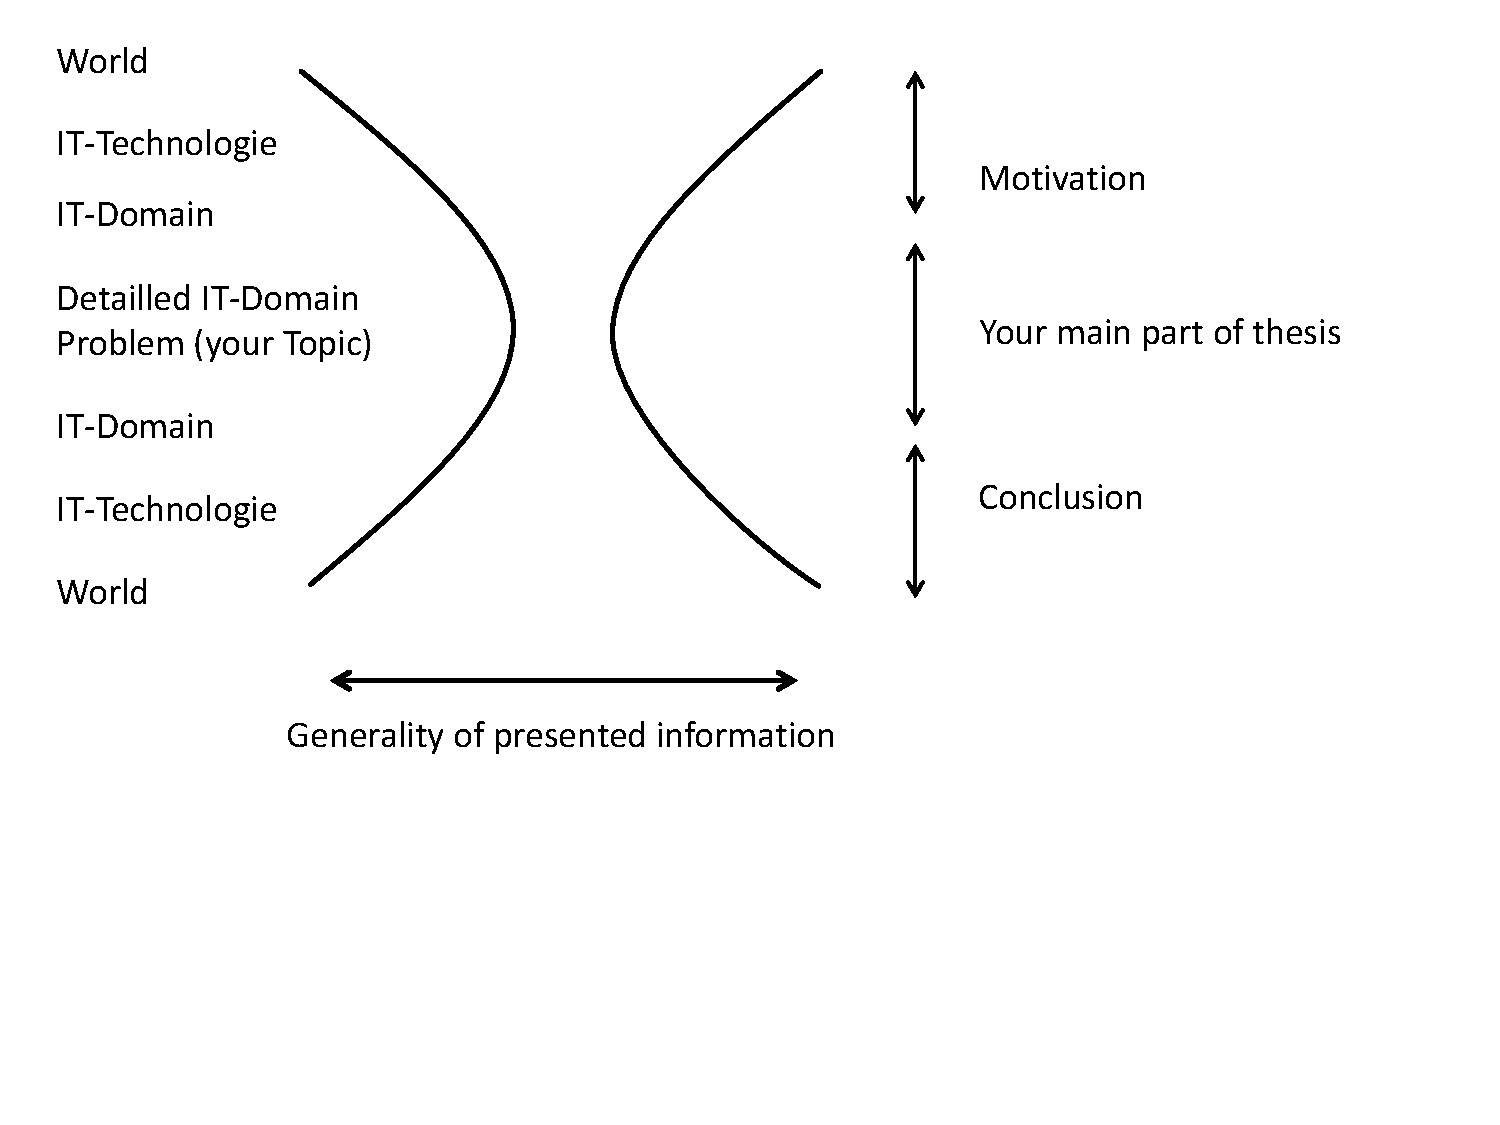
\includegraphics[width=0.9\textwidth]{template/writing}
%\caption[Information Generality]{This images illustrates how generality of information could be handled in a thesis. In your motivation you should start from a very broad view on the topic. Then you should get more precise with every statement until you reach the actual problem you are addressing. You should do vice-versa in your conclusion, starting with the problem that you addressed and getting broader until you can write about the meaning of your results to the (IT-)world.\label{fig:writing}}
%\end{figure}







%###################################################################################
%###################### Approach and Goals  ########################################
%###################################################################################
\section{Approach and Goals}
%DELETEME: In this section, you should cleary describe your approach that you are following in order to solve the underl*a*ying problem of your thesis. Additionally, you should clearly state the goals of your work. This will not only help you supervi*z*or to understand what you are doing, it will also help you to be sure on which topic you should evaluate.





\todo{\textbf{Aufgabenstellung:}\\ 
	-AL: Anschlie{\ss}end soll das Ziel der Arbeit formuliert werden: Entwicklung und Evaluation eines Prototypen f\"ur den Anwendungsfall.\\
	\\
	1- es sollen die St\"arken und Schw\"achen eines solchen System zu analysieren. 
	2- Es sollte zun\"achst eine Dienstleitung aus dem Berliner Service-Katalog mit dem Chatbot \"beauskunftet\" werden k\"onnen.\\
	3- Nuancen beachten (e.g. 10243 / FHain)\\
	4- Smalltalk F\"ahigkeiten
}

\todo{
- ..it would speak as an advantage for bots if they can determine these things automatically..\\
%	mentioned earlier - imagination about ablitiy to react to everything\\
- currently most tasks revolve around performing tasks like setting an alarm, 
%	to perform task like - mention top 10 and a few more stats / tech review
- answer suggestions functionality in chatbot equivalent
- next step is to get around the user's frustration by making the bot at least more human.	

- Alexa Skill will work in Germany in english and german -> add english after german
}


%###################################################################################
%###################### Structure of the Thesis ####################################
%###################################################################################
\section{Structure of the Thesis}
%DELETEME: This section does not require eloquent writing. It is just a presentation of what you will handle in each chapter starting with Chapter~\ref{background}.
%

This thesis endeavours to shed light on the following: In Chapter~\ref{background}, we discuss related work as currently available. We first show a few use cases for chat bots and voice assistants and their implementation. For that we consider \inote{the City of Vienna chat bot service \href{https://www.wien.gv.at/bot/}{''WienBot''} for German and Singapore/ \href{http://www.govtech.com/7-State-or-Local-Governments-Using-Amazon-Alexa.html}{LA/...} for English} and compare them to the current application available on \href{https://service.berlin.de/virtueller-assistent/virtueller-assistent-606279.php}{service.berlin.de}.
We then introduce the Alexa platform and the idea behind Skills in chapter~\ref{mainone} and discuss how it can overcome a few struggles with respect to its counterparts \inote{like redundant boilerplate code, smalltalk, but also limitations}. We also present the frameworks we use in our own implementation, the prerequisites and the artefacts provided initially.
Chapter~\ref{mainone} and~\ref{maintwo} represent a detailled analysis of our implementation. In particular, \inote{SOME MORE SENTENCES.
In Chapter~\ref{maintwo}, our solution is presented. This solution covers ... (SOME MORE SENTENCES).}
Chapter~\ref{evaluation} evaluates our implementation with respect to our target in the defined \inote{4-5} use cases. \inote{SOME MORE SENTENCES}
In Chapter~\ref{conclusion}, we conclude with how the implementation of this e-Government solution is attainable through Alexa and where future works can be directed. 
%Chapter~\ref{appendices} gives additional related information on the topic of this thesis.}
%to head
%\chapter{Background}
%%labels will help you to reference to certain images, tables, chapters, section, and so on...
%\label{background}


\chapter{Background and Related Work}
\label{relatedWork} 





%DELETEME: This chapter will cover all of your background information and related work. Background and related work are directly related to your thesis. Please do not place irrelevant content here which is a common mistake. Citing will be handled in the appendices.

%\todo{check the label with the old and new texts after restructure}


%In this chapter we discuss Amazon's state-of-the-art strategy
%%before moving on to related work in other archetypes 
%as it is important to introduce the implementation scope of voice assistants 
%top down
%%bottom-up 
%prior to exploring the current context 
%%within the same boundaries of voice assistants 
%%then 
%after comparing it to other approaches in the larger context of conversational bots as a whole from a technical and user experience point of view. 


%moved to gui section
%We start with a juxtaposition of Voice User Interface (VUI) to the Graphical User interface (GUI) respective to cognition and behavioural design which gets us to define new terminological foundation that will follow throughout this thesis.

%moved to chapter 3: to then elaborate on implementation requirements in Section \ref{frameworks_structs}. 


%DELETEME: Background represents underlying knowledge that is required to understand your work. The expected knowledge level of your readers can be set to the one of a bachelor or master student who just finished his studies (depending on what kind of thesis you are writing). This means that you do not need to describe how computers work, unless your thesis topic is about this. Everything that an avarage alumni from your field of studies should know does not need to be described. It turn, background information that is very complex and content-wise very near to you problem, can be placed in the main parts. Everyting else should be written here. Note: it is important to connect each presented topic to your thesis. E.g. if you present the ISO/OSI layer model you should also write that this is needed to understand the protocols you plan to develop in the main parts.







%#############################################################################
%###################### Related work (Bkgrd) ########################################
%#############################################################################

%DELETEME: Related work respresents results from work that handled the same or a similar problem that you are addressing. This work might have used a different approach or might not have been that successful. Finding a paper / work that solved your problem in the same way you were planning to do is not good and you should contact your supervizor for solving this issue. Again, each paper / work has to be connected to your approach: other papers might have not chosen an optimal solution; they might not have been taking care of essential aspects; they might have chosen a different approach and you believe, yours will work better ...

%\chapter{Related Work}
%\label{relatedWork}

As our motivation stems from the unstoppable worldwide trends of digitalisation, in this chapter we discuss current application categories
with respect to chatbots and voice assistans
and talk about governments' efforts in keeping up with these trends as part of their 
modernisation stream
%technology streams 
%in governments 
in the age of social media, Internet of Things (IoT) and the interaction between both.
We then show relevant examples in our context of voice assistants.




\section{Topology of Chatbots and Voice Assistants}

Chatbots and voice assistants come in numerous mouldings; on the web, in apps, through smartphones or as a combination of those and beyond. In Barot and Oren \cite{guidetochat} we observe the different purposes the industry caters for. As we witness the integration of chatbots in retail, productivity, entertainment and create more possibilities for their existance, it is obvious that the trend will continue for a while before the market is saturated. Similar to marketplaces for applications like Apple's App Store and the Google Play Store which have become a commonplace term even though their slow stagnation in the recent years, chatbots and voice assistants are predicted to remain trendy for some time as VoiceLabs predicts (Figure \ref{voiceLabs:mktpreds}). Moreover, SearchMetrics advises on SEO tweaks for Google Voice Search \cite{searchmetrics:blog} show how voice assistants are becoming a ubiquitous market.


%ssssssssssssss

Google Actions
%ubiquity of voice
%searchmetrics report


\todo{%move / remove what is irrelevant
	%	In this section, we conduct a short survey of problems we can face with natural language
	
	
	\textbf{by category}\\
	- leisure /
	- \href{https://www.forbes.com/sites/tomaslaurinavicius/2017/04/24/facebook-messenger-bots/\#4f61c16a66d8}{fun bots}  / 
	- productivity / 
	- more (graph from voicelabs report) \\
	- what are classic use cases for their use with prominent examples?\\ Booking tickets (e.g. airline bot)\\ %KLM
	- quick survey of respective 'AppStores'\\
	\textbf{by purpose}\\
	-physical locations (home, office, car, phone, in a business)\\
	Information bots\\
	\textcolor{magenta}{
		- mention available service types (information system as a "webpage/database")\\
		- vs an interactive bot that gives you customized information on demand
		hier soll der D115 Anwendungsfall "Beauskunftung" kurz erl\"autert werden\\
	}
	social bots\\
	\textcolor{magenta}{
		- with advantages / disadvantages\\
		- fake news / online reviews\\
	}
	more on AI in bots (optional)\\
	\textcolor{magenta}{
		- use of ML\\
		Handyversicherungsbeispiel\\
		- from business perspective, the bot is aiming to sell more polices,\\ 
		- the bot tries to determine if there is a nuance in the user's answer (machine acting as a judge!)
		- e.g. ``how did the phone fall off``
		- MKTG - Aufwand
	}\\
	IFTTT Applets for voice commands\\
	IFTTT didn't work because it was semi automated. you needed to zwischgreifen (Ivo Lehrter)
}













\section{Digitalisation in the Public Sector}

There is no doubt that social media has changed the shape of our society in the last twelve years. Not only by affecting the way we communicate, but also by generating immense amounts of data, creating new jobs and disrupting economies en masse.
Meanwhile, governments are continuously striving to market their image in more creative ways than ever to target more segments in society. From what used to be a novelty, politicians' tweets are now a highlight in main news sections. The sudden interest of governments in social media platforms 
can be seen as an attempt to become more transparent and reach more public awareness. It is more likely for instance that a 15-year old would find out about a public figure (including a president) by following their story on Instagram than by reading news about them on dedicated news website.

This is ultimately because the social media platform, as part of many new technologies are designed with the focus of reach in mind much more than only availing information to the target.
We distinguish between the pull-based model of information retrieval, where a person would actively look for certain information usually through looking something up, vs. the push model, where the information is `thrown' to the user without them actively asking for it, usually by subscribing to the source or news outlet and more likely through audiovisuals than trough text. Unsurprisingly, such platforms become a key player in redefining fame, identity and image.

The push-model is a new strategy to dissemination of knowledge, which governments %also decided to 
embrace \cite{forbes:govOutreach} to bridge the gap in their outreach to the public. 
Although the digitalisation trend in governments generally emerges from the desire to expand infrastructure for information exchange and availing open government data \cite{un:egovReport}, digital media has now become an integral part of it, too, making it inseparable from many institutions compositions. 

In Germany, many advanced milestones in digitalisation were attained in the last years. From eliminating paper in many administrative workflows 
%in government bodies %sssssssssss
to funding successful start-ups in the field (e.g.Aaron.ai \cite{exist:aaron})
and seeking renewable energy as a foundation %of scale 
to power an exponentially growing number of devices in the country with a reduced carbon footprint, the aspect of digital media has been relatively neglected compared to other countries.
According to numbers from the United Nations' E-Government Development Index in 2016, Germany ranked 15th worldwide and 8th within Europe with an average of 0.82 % of its services provided or operated digitally 
, substantially outranked by the United Kingdom, the United States, Singapore and France. Outperforming its previous statistics from 2014 where its index scored  0.79 with a world average of 0.47, where it was also outranked by Austria, Israel and Bahrain \cite{freiheit:digitalisierung} in addition to the aforementioned countries as listed in Figure \ref{un:egci}.  Germany's ranking went up from 21st to 16th worldwide in the last two years.

\begin{figure}[h]
	\caption[E-Government Development Index in Europe]{Top Ten Countries for E-Government Development Index in Europe based on \cite{un:egovReport}}
	\label{un:egci}
	\includegraphics[width=\textwidth]{Govcharts/TopTenEUeGov} 
\end{figure}


the E-Government Development index (EGDI) is composed of a calculation based on proportionally normalised averages of the Online Service Index (OSI), the Human Capital Index and the Telecomunication Infrastructure Index. 
%as can be seen from Figure
When it comes to engagement through e-participation, Germany performance lies also in the top quartile. Its Online Service Index performed 21st worldwide (Figure \ref{un:osi}), which shows the continuous strive to maintain relatively many rights to access government information online and an open data government policy on the web.

\begin{figure}[h]
	\caption[United Nations Online Service Index (Top 30)]{Online Service Index for Top 30 Countries Worldwide based on The UN Department of Economic and Social Affairs \cite{un:egovReport}}
	\label{un:osi}
	\includegraphics[width=\textwidth]{Govcharts/osicopy} 
\end{figure}

In an age where we
take the internet for granted,
we also expect to have multiple communication channels open to government representatives and public authorities. 
%just like we 
%it for granted to be able to check flight delays on a designated platform, we also expect to constantly have immediate access to a communication channel with local and global representatives.
%
%Governments targets in social media have become  digitalisation 
%it started with social media-now want to give a face and experience(kan2oho sherka) not only by eliminating paper 
% eliminating carbon footprint. almania w heya gamda keda w bte3mel atomkraft nein danke
%\todo{bring up the Freiheit.org chart \cite{freiheit:digitalisierung}\\ 
%	Talk about digitalisation in general (how there are talks in DE about autonomous driving and the related regulations - ref Haase)\\
%	say that \\ bass}
Hence, out of public interest, governments are advised not only to focus on digitising their internal structure, but also their representation on the public sphere.
Especially at times of change like with the introduction of autonomous driving and the regulations related to it, transparency is a continuous expectation from the people. As stated above, since transparency heavily relies on public presence, which in turn depends on availing more communication platforms, voice assistant services are definitely worthy of consideration in that context.




\section{Worldwide Examples of Bots in E-Government}

Knowing that the Online Service Index of a country consists of the services available to different groups of society, we can argue that 
%it is also important to acknowledge how 
vulnerable groups (i.e. the poor, persons with disabilities, older persons, immogrants, women and youth) can be easily marginalised in this index. Another statistic by the German Federal Statistics Office (Statistisches Bundesamt) shows that most online public services in 2016 were targeting persons of age 25-44 with an equal offer of services for age groups 45-67 and 16-24 with the least amount of services targeted at youngsters between age 10 and 15 comprising 15\% of the service catalogue (Leistungskatalog, LeiKa) \cite{stabunda:leika}.
For that reason, we acknowledge the importance of inclusion especially towards vulnerable groups in the process of expanding a online public service.

This gives us the advantage to promote in the development process of a chatbot or a voice service assistant for inclusion especially since the domain is relatively still uncharted. As Zehlike et al. conclude, given the many possible biases Machine Learning Algorithms can result in \cite{fa:ir}, a holistic approach is required to have a balanced distribution of services in different fields (e.g. Health, Finance, Administration) for different groups of society (protected and unprotected groups).
%(children, elderly, foreigners, locals, immigrants, men, women, youth).
Already offering a service on platform that offers less constrains to the user than a browser's graphical user interface (GUI) allows per se more options for inclusion but could also be limiting of the system reacts to a vocabulary used only by a certain group for instance.

In terms of functionality and testing of a chatbot or voice assistant system on inclusion metrics, WitLingo \footnote{\url{https://www.witlingo.com/}}, a company which builds voice-driven apps for banks, universities, law firms as well as other public and private sector enterprises believes in that sense that ``getting feedback [on the performance of the voice service to different groups of people] is more important than measuring ROI'' \cite{witlingo:bouzid} with a report that reflects the same statement in the retail sector from Voysis and Retail TouchPoints \cite{voysis:report}.


%sssssss

%\todo{
%%	WitLingo: which builds voice-driven apps of all sorts for banks, universities, law firms, and others.\\
%%	aaron.ai use cases (local examples)\\
%%	
%%	\textbf{eingehen auf} Singapore / LA /.. as cities that have a higher index of e-gov and use chatbots\\
%
%%	say you chose wienbot and askgeorgia as german and english counterparts
%}


	While there are several cities such as Singapore and Los Angeles integrating chatbots and voice assistants into their administration's websites and coming up with all sorts of interactive solutions,
	for this research we choose the City of Vienna chatbot service \href{https://www.wien.gv.at/bot/}{\textsc{WienBot}\footnote{\url{https://www.wien.gv.at/bot/}}} given that it uses German 
	and the Alexa Skill \href{https://www.amazon.com/GeorgiaGov-Interactive-GTA-Ask/dp/B074XBQGTQ}{\textsc{GeorgiaGov}}\footnote{\url{https://www.amazon.com/GeorgiaGov-Interactive-GTA-Ask/dp/B074XBQGTQ}} for a comparison in US English, as we examine both languages in our development process.

\subsection*{\textsc{WienBot}}
developed for Vienna, Austria
	mention who they are developed by etc. Aquaponics etc
\todo{pics of interface and conversation}




%\todo{
%	\\
%	Ask GeorgiaGov is developed by that company (get source)
%}
\subsection*{\textsc{GeorgiaGov}}
developed for Georgia, USA
	mention who they are developed by etc. Aquaponics etc
\todo{pics of conversation}

\begin{quotation}
The state of Georgia has always been on the forefront of web accessibility. For example, from 2002 until 2006, Georgia piloted a time-limited text-to-speech telephony service which would allow website information and popular services like driver's license renewal to be offered to citizens \cite{dries:georgia}
\end{quotation} 


	While we are less interested in the content delivered through the voice assistant and have no access to AskGeorgia from the German Amazon Store, we use the US store for our conversation testing purpose to pick the relevant design of flow of conversation. %tab3an di f amrika fal mawdou3 mokhtalef, bas el fekra here is el design not the exact content






















%###################################################################################
%###################### Use Case in detail  ########################################
%###################################################################################
\section{Berlin as a Use Case}
\label{blnusecase}
As Schwarzer et al. state, few systems are available that ``enable Berlin’s citizens to inform themselves of governmental services'' \cite{lomm:gov}.
As part of the modernisation process, the \textsc{Virtual Citizen Assistant (Virtueller Bürgerassistent)} was born in \inote{developed by} the Information Retrieval and Machine Learning Competence Centre of the Technical University of Berlin's Distributed Artificial Intelligence Laboratory.



\todo{
	- structure of Hitlist on berlin.de  is provided by ITDZ -  as opposed to Versicherungsfirma z.B (ML tries to detect irregular patterns in case customer is lying).
	- unfortunately forums vs. FAQs did not work. if i want assistance, i want the customer to tell me the model number - and forums have mostly Schrott!\\
	what the bot curently achieved is at least not give wrong answers, sometimes says idk but it doesnt confuse u. same attitude like in lmny shops (nur unpassende antworten sind frustrierend!\\
}





%\subsection*{D115 and The Currently Deployed ``Virtual Bürgerassistent''}
\todo{
	- LeiKa
	- summarize infobroschuere\_ BMI08324\_screen\_barrierefrei.pdf\\
	-Use case im Detail\\
	-Welche Daten gibt es?\\	  
	-Was sind die Erwartungen?\\ 	
	- wie kann man die G\"ute des Systems beurteilen? \textbf{do not forget the surveyu made}\\   
	- Meist sollte man in diesem Kapitel die L\"osung schon im Auge haben, um die Erwartungen so zu formulieren, dass die L\"osung auch geeignet ist?\\ 
}


\todo{
say that the bot is developed as a webapp using groovy.\\

if anything about AllInclusive is to be mentioned, it should go here or before it can go in implementation section.\\

We cover here an excerpt of basic elements that we will later see more or less in the same structure of the JSON file containing the interaction model:\\


}

\todo{
	\textbf{current berlin.de bot}\\
	- dienstleistungen.json structure (finding the info through hierarchical nodes)\\
	- interpreting the nodes as intents\\
	- traversing the nodes (one level up then to next node)\\
	- no session/no persistence\\
	- explain how the json nodes map to intents and cores in solr etc
	
	%x	x	x
	%ooo ooo ooo
	%try first, go to second (kosten, zeit, rechtsgrundlage, ..) skip one if it has already been suggested.. hinweis..that is built into the xml
	%
	%the live service is different than the one at DAI
}

%%%%%%%%%%%%%%%%%%%%%

%\Tree [.Dienstleistungen.json created [.VP [.V is ] NP ] ]
%
%\Tree[.Dienstleistungen.json 	
%	[.NP [.Det \textit{the} ]
%		[.N\1 [.N \textit{package} ]]]
%	[.I\1 [.I \textsc{3sg.Pres} ]
%		[.VP [.V\1 [.V \textit{is} ]
%			 	   [.AP [.Deg \textit{really} ]
%				  		[.A\1 [.A \textit{simple} ]
%							  \qroof{\textit{to use}}.CP ]]]]]]]





\begin{figure}[h!]
	\caption{\mintinline{java}{Dienstleistungen.json}  - Primary Nodes}
	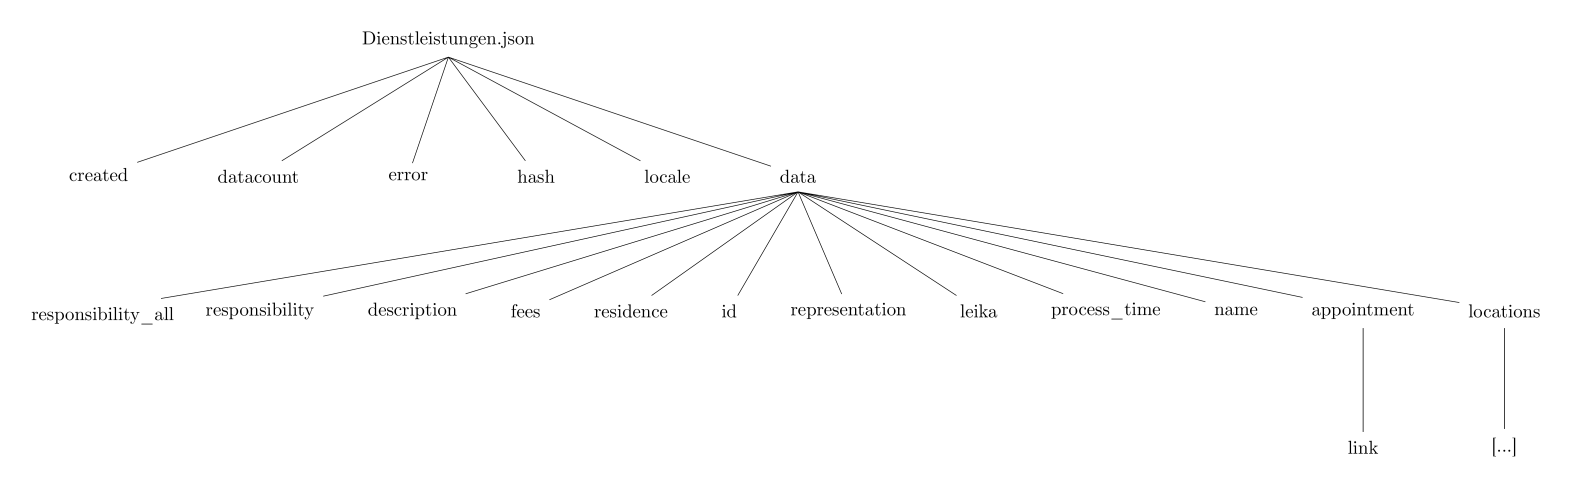
\includegraphics[width=\textwidth]{DLprim}
\end{figure}

\begin{figure}[h]
	\caption{\mintinline{java}{Dienstleistungen.json} - secondary Nodes}
	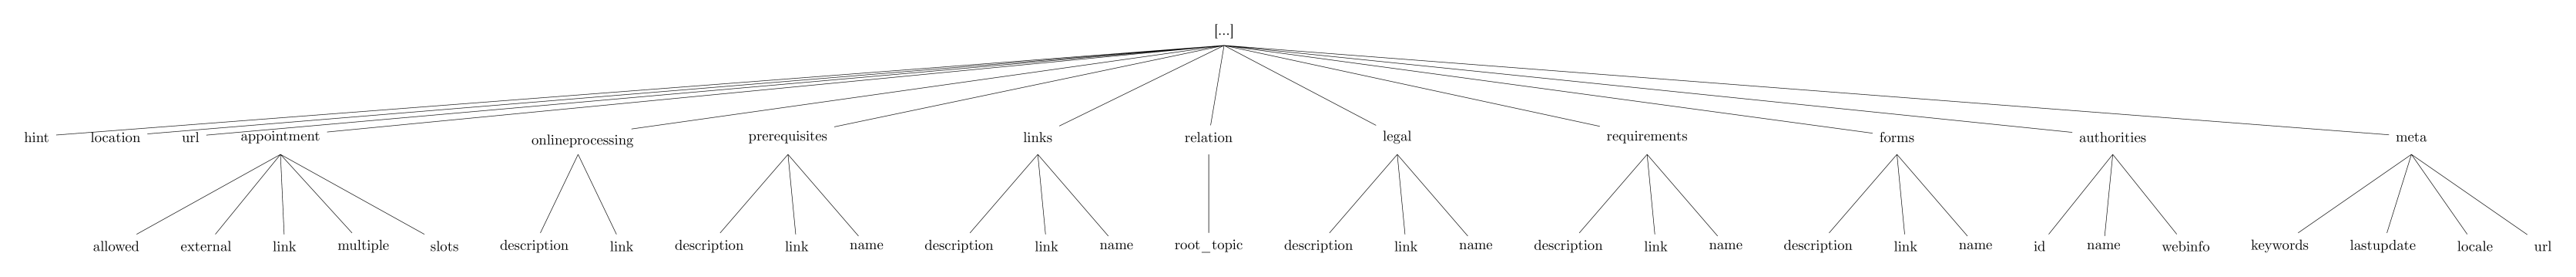
\includegraphics[width=\textwidth]{DLsec}
\end{figure}



provided in JSON for value lookup, the structure of the file is as follows: there are \inote{carry on - the structure}


started with 616 Intents in \lstinline|data| node (now 685 or so), each containing \inote{}
\todo{missing variables e.g. are required papers, flag: persönliche Vorsprache ja nein, ...}
\todo {change this into a table and add a tree list like the interaction model in appendix}

\begin{table}[htbp]
	\caption{relevant nodes in query results \mintinline{java}{Dienstleistungen.json} - Description}
	\label{dienstleistung:descr}
	\begin{tabu} to \linewidth {  r | l | l | l }
		key & type & ex. Value & description\\ \hline
		
		\mintinline{json}{id} & \mintinline{json}{int} & 326233 & public service ID on \href{https://service.berlin.de}{service.berlin.de} \\
		
		\mintinline{json}{d115URL} & URL \mintinline{json}{string} & ''https://service.berlin.de/dienstleistung/326233/'' & link to public service URL on  \href{https://service.berlin.de}{service.berlin.de} \\
		
		\mintinline{json}{d115Name} & \mintinline{json}{string} & Fiktionsbescheinigung & public service name as listed on \href{https://service.berlin.de}{service.berlin.de/dienstleistungen} \\		
		
		\mintinline{json}{ssdsAll} & \mintinline{json}{string} & ... & additional captive search terms, synonyms used by Virtueller Bürgerassistent. Found to be helpful in conversations with the chatbot \\		
		
		\mintinline{json}{d115Description} & \mintinline{json}{string} & ... & Introductory paragraph from the service web page. 
		Includes HTML tags \\ %like <\backslash br> and <ul ...> \\		
		
		
		%		
		%		\mintinline{json}{d115Synonym} & \mintinline{json}{string} & ... & captive search terms, synonyms created by Virtueller Bürgerassistent \\		
		%		
		%		\mintinline{json}{d115Position} & \mintinline{json}{string} & ... & captive search terms, synonyms used by Virtueller Bürgerassistent \\		
		%		
		%		\mintinline{json}{d115InfoLaw} & \mintinline{json}{string} & ... & Legal base for offering this public service \\		
		%		
		%		\mintinline{json}{ssdsAll} & \mintinline{json}{string} & ... & captive search terms, synonyms used by Virtueller Bürgerassistent \\		
		%		
		%		\mintinline{json}{ssdsAll} & \mintinline{json}{string} & ... & captive search terms, synonyms used by Virtueller Bürgerassistent \\		
		%		
		%		
		%		
		%		
		%		
		%		
		%		
		%		\mintinline{java}{string} & \mintinline{java}{responsibility}  & denoting in which city halls a service is available\\
		%		\mintinline{java}{boolean} & \mintinline{java}{responsibility_all} & a flag set to true in case the service is available in all local authority offices / service points\\
		%		
		%%	\mintinline{java}{HTML list string} & \mintinline{java}{ description} &  not unified and includes text \\
		%%%		\item  \lstinline|<string> not unified and might need to have an \lstinline|int| added to it and set to 0 in case service is free
		%		\mintinline{java}{int} & \mintinline{java}{residence} & \\
		%		\mintinline{java}{int} & \mintinline{java}{id} & \\
		%		x & \mintinline{java}{representation}  & x\\
		%		\mintinline{java}{long} & \mintinline{java}{leika}  & \\
		%		\mintinline{java}{string} & \mintinline{java}{process_time}  &  need to derive minimum, average and maximum service times instead of a string, as well as conditions\\
		%		\mintinline{java}{string} & \mintinline{java}{name} & the name of the service that would make sense to a human \\
		%		\mintinline{java}{node} & \mintinline{java}{appointment}  &  \\ 		
		%%		% then inner node 
		%%%		\begin{itemize}
		%%%			\item \lstinline|link| (Key value with URL to /terminveinbarung page) - check if orphan or if it is for each beh\"orde and in that case how it gets the right one
		%%%		\end{itemize}	 
		%		\mintinline{java}{node} & \mintinline{java}{locations}  & \\ 
		%%		% then inner node
		%%%
		%%			\mintinline{java}{hint}
		%			\mintinline{java}{int} & \mintinline{java}{sth} & location| one of the 12 authorities \\
		%%%			\item \lstinline|url| of that service at that authority
		%			\mintinline{java}{node} & \mintinline{java}{appointment} & (a second one)	 \\	
		%		\mintinline{java}{node} & \mintinline{java}{onlineprocessing}  & \\
		%		\mintinline{java}{node} & \mintinline{java}{prerequisites} & \\
		%		\mintinline{java}{node} & \mintinline{java}{links} & \\
		%		\mintinline{java}{node} & \mintinline{java}{relation}  & \\
		%		\mintinline{java}{node} & \mintinline{java}{legal}  & \\
		%		\mintinline{java}{node} & \mintinline{java}{requirements}  & \\
		%		\mintinline{java}{node} & \mintinline{java}{forms}  & \\
		%		\mintinline{java}{node} & \mintinline{java}{authorities}  & \\
		%		\mintinline{java}{node} & \mintinline{java}{meta}  & \\
	\end{tabu}
\end{table}














%#################################################################################
%###################### State of the Art  ########################################
%%#################################################################################
%\chapter{State of the Art}
%
%\sn{intro sentence}
%
%







%###################################################################################
%###################### Topic B             ########################################
%###################################################################################

%% moved to Chapter 3


































%###################################################################################
%###################### GUI/VUI ####################################
%###################################################################################

\chapter{The Voice as a User Interface} 
\label{vui}


We start with a juxtaposition of Voice User Interface (VUI) to the Graphical User interface (GUI) respective to cognition and behavioural design which gets us to define new terminological foundation that will follow throughout this thesis.

\section{GUI vs. VUI}
\label{guivsvui}

Visuals and Sounds can both communicate the same message even though they use a  completely different medium. One one hand, the premise that ``a picture is worth a thousand words'' can be valid based on the image but only assumes that we want to give a clear picture to the receiver. Communication through voice, on the other hand, can generally allow more room for interpretation. We think of an example where you would watch a football game on TV vs. the same game on radio, where listening to it allows each person in the audience group to imagine a different game for themselves, even though the match result are the same.


%%%Image

When we use written text, be it in a document or a street sign, or any label, we seek to mostly assure that all receivers understand the same message with a universal codification of what we want to express through the language we use. In this process, language becomes the common denominator for understanding and the short written text becomes purposefully designed to give in the best case a message not open to interpretation and so a foundation for an agreement or contract between the source and the destination of the message. It is a good medium of reference. 

%%%%%%%%%%%%%%%%%%%%%%%%%%%%%%%%%%%%%%%%%%
%voice message in airport - you can do your activity unobstructed
%%%%%%%%%%%%%%%%%%%%%
\section{Utility of Voice}
The utility of Voice comes handy with its different paradigm in numerous settings. 
For a passenger at the airport or an employee between meetings, 
%it is equally as helpful f
%as it would be for a  rushing to a meeting.
it can be more effective to ask questions through conversation than transform them into a query then type them on a screen,
%someone about the information you need quickly if you can ask it in a precise sentence quicker than you would write it, 
or visually navigate on a web page / mobile application until we reach the information we want. In a 2016 Cisco Systems (formely MindMeld) survey \cite{mindmeldReport}, of 1800 users of voice assistants, 61\% see that the primary use of a voice assistant is when hands or vision is occupied.
Today, this goes further beyond the simple use-cases to become an integral part of our fast-paced life, where we see companies like Ecobee getting around 40 percent of their sales through voice-based AI \cite{mit:Alexa} since their embrace about two years ago. The 10-year-old company's CEO elaborates that their customer “[...] have to fight traffic to get home, and then they have to feed the kids, diaper the baby, and who knows what else. [Ecobee] give them a hands-free way of getting something done while they’re in the midst of other tasks.”


Also, in terms of accessibility, blindness could sometimes make voice the only possible way to navigate or be aware of one's surroundings, e.g. a blind person crossing a street depends on the sounds coming from cars and traffic lights.
In that sense, voice can allow people to do their activities free-handed and unobstructed by actively engaging into reading activity, for instance having to look on a screen.
As our ambitions in connectivity become more complex, we have become more dependent on our phones in the last decade.
This is where use of a Voice User Interface could have the advantage of liberate us from the constant usage of our smartphones and moving from one screen to another. 
However, it is noteworthy that the trade-off between information exchange visually and through audio comes at a price. While both have their own advantages and disadvantages, it is important to understand that the context in which the medium is used is an important factor.

Hence, we need to differentiate between GUI design and that of a VUI. Since  we come from a GUI background thanks to the World Wide Web standards with HTML and CSS, it might not be most intuitive to apply the same concepts on VUI design simply since we start from the mindset that the GUI dictates how to use the software and the user has to understand this interface and deal with it as is.




\todo{ghaleban mesh mazbouta hena ba3d el refactoring eli 7asal}


%\inote{is this okay here or should it go in an appendix?}
%\sn{andreas doesn't like to have more work done in this part. maybe put some of it in conclusion or remove completely, but i know you won't lol}

\section{Why Can't AI understand us}

AI has made giants leaps in the last few years. Thanks to neural networks, bayesian approaches in classification, decision trees and many other theories, we are capable of performing rigorous analyses on datasets
Considering that speech is one of the most complex forms of such, there are still various challenges that do not have a single strategy to tackle.

\begin{quotation}
What makes voice-based AI so appealing to consumers is its promise to conform to us, to respond to the way we speak—and think—without requiring us to type on a keyboard or screen. That’s also what makes it so technically difficult to build. We aren’t at all orderly when we talk. Instead, we interrupt ourselves. We let thoughts dangle. We use words, nods, and grunts in odd ways, and we assume that we’re making sense even when we aren’t \cite{mit:Alexa}.
\end{quotation}

When speech meets AI, there are a lot of language ambiguities to deal with and multiple contexts to understand. Since this is a field by its own and the amount of problems we can face with understanding natural language is unlimited, it is not the scope of this thesis. We only briefly survey a few categorical examples in the following:
\begin{itemize}
	\item \textbf{Sytanx}: homonyms such as ``I \textit{present} you a \textit{present}.'' or ``The \textit{fly} wants to \textit{fly}''
	%homophones, homograph
	
	\item \textbf{Sematics}: metaphors, sarcasm, puns such as ``it’s raining cats and dogs''
	
	\item \textbf{Underlying Sentiment}: such as ``oh yeah, sounds very exciting'' when it's not.
	
	\item \textbf{Dialects}: enunciation such as \textipa{[dI"vE|9pm9nt]} \textit{(British)} and \textipa{[d9v"|Apm9nt]} \textit{(Indian)}

\end{itemize}

%\end{itemize}
%
%\begin{table}[h]
%	\begin{tabularx}{\textwidth}{r l l}
%		Syntax & Homonyms & \shortstack[l]{``I \textbf{present} you a \textbf{present}.''\\ ``The \textbf{fly} wants to \textbf{fly}''}\\
%		Semantic & Metaphors
%	\end{tabularx}
%	
%\end{table}
%

%\todo{
%	- \textbf{Why can't robots understand us:} language ambiguities - the need to understand context\\ the facebook vid\\
%--Syntactical: Homonyme\\ %fly, fly,  presently I’ll present you a present - now, give, gift
%--Semantic:  Methaphors, %“it’s raining cats and dogs”
%sarcasm, %“oh yea, sounds very exciting”
%and puns\\
%--dialects: enunciations\\
%--underlying grammar\\ %“what makes you abcd just now, ELIZA
%--underlying sentiment\\

%-\textbf{NLP Progress:} How does it help in enriching the bot experience\\
%--neural networks: help understanding language patterns and get better over time\\
%--thought vectors: helps connect different words with related meaingns\\
%--- link: fortschritt, und systemgrenzen heutzutage (kurze Sätze etc)
%}

While Machine Learning enables us to decode phrases not in the classical way in the past by randomly guessing the whole expression, our speech datasets grow and require analysis in further breadth and depth to deliver a sustainable Natural Language Understanding (NLU) engine.
So far, in the past six years our primary approach has changed due to the little progress made with it. Instead of trying to understand exact meanings, we work from
``imperfect matches at the outset, followed by rapid fine-tuning of provisional guesses'' \cite{mit:Alexa}. The learning part is involved by reinterpreting missed expressions \cite{aws:lex_webinar}. 
On one hand, neural networks help us understand language patterns and better the more frequently we use them, but can fail in the case of homonyms. \cite{mit:AILang} Thought Vectors on the other hand complement them by controlling the connection of different words with their related meanings %, which helps with homonyms for instance.

Depending on the system, it is therefore a rule of thumb that most AI-powered personal assistants like Siri or Alexa are in their early learning phases. In order to be able to make use of them in the future, the painful immaturity part has to come in effect. This limits us for instance to using short sentences to lessen the probability of the system misunderstanding us. And so, naturally, what distinguishes a good system from a better one is how fast it learns.


%a person whos a bit deaf and cant hear us. it happens with ppl too ya3ni}
Interestingly, a side effect of this indeterministic technique is that the voice assistant inadvertently simulates a person, who can sometimes not hear us, asks us to repeat a sentence or explain it in a different way. Although this is the same idea that a good system should have minimal fault tolerance, it is unprecedented to tackle a computer system on the consumer level with the idea that we might very much hit or miss the action we want to perform. On the other hand, though premature, it is evidence that a human has much more authority to a machine-powered brain.


Yet, although it might seem at the beginning that moving between both paradigms is easy, the more detailed system design gets, the trickier it becomes to transform GUI elements into text. Particularly with long texts. We will go over this in more detail about voice design guidelines in Section \ref{designGuide}.



\todo{ 
	this is a refactored todo. read in context and see if it fits here\\
%	2 \P \\
	
	\textbf{- Chatbot vs. human: }
	%what we used to do with facets vs a search mask predicting possible facets - we are at a stage where bots are like altavista..u tell alexa to open a skill like u tell altavista to look in pics or go to lexisnexis to do reserach. we are yet to reach the state of watson like google is to searches
	Analyze differences between bot and human response\\
	%human says long sentences and there is a fluid transition between dialog and monologue 
	-disadvantage: a bot wants a sentence broken down in small pieces to avoid errors in lengthy interpretation\\
	% otherwise, error margin too large.\\
	% this has to do with human language complexity.\\
}



\section{VUI Semantics}

Having the visual or haptic interface disappear is therefore a game changer for as soon as the user does not have direct instructions on how to deal with it, they start to improvise, or rather move away from the idea that the interface constrains them to the illusion that they define that interface and can control it. For instance, the user knows that they have to press only on a certain area of the screen to activate a button and actively move the mouse to that part. 
%Parallel to this in GUI; 
In other words,
when a user sees a  `save' button on a dialogue box, they relate to it in their head that the functionality behind that button lies in committing and keeping a persistent copy of the current state of the parent file to that dialogue. The label `save' describes in a visually expressive fashion what the user can or cannot do within this \textit{dialogue state}.


%Imagine you have an intent resembling the label on th button for ``ok''. with a function linked to it to perform a commit action, ...''}
%  

In voice on the contrary, a user is uninhibited in what they can and cannot say and the system is supposed to understand the \textit{intention}%~\ref{intents} 
of the user with \textit{the formulation}%~\ref{utterances} 
they just used.

%For us to hold on to that sentence, 
In order to translate the aforementioned with less ambiguity, we need to define the lexis we use for voice design utilized in most common chatbot and voice assistants constructs. 
%Just like most common chatbot constructs, Alexa Skills Kit (ASK) 
We divide the building model into intents%~\ref{intents}
, utterances%~\ref{utterances}
 and slots %~\ref{slots}. 
The Fulfilment part is taken care of through a back-end endpoint containing the programming and business logic to the interface, which also validate the slots before sending it onwards, similar to what JavaScript checks would do on a website. %We make the following words clear:

%\sn{Andreas suggests hochstufen - clear split required?}
\section{Terminology}
%Before we discuss our choice of platform in Section \ref{choiceOfPlatform}, 
We already unveiled in Section \ref{approachgoals} that Alexa will be the underlying system. Thus we cap the elementary definitions of voice assistants with distinct Alexa-specific concepts and give meaning to the following terms: 

	\subsection*{Intent}~\label{intents}
	As the intention the user pursues with a spoken sentence. This translates to the action being executed upon the user's command based on mapping his/her words to this action.
	
	\subsection*{Utterance}~\label{utterances}
	As the wording a user picks to express his intent. For instance, to set the volume on a TV to quieter, we could say ``turn it down a nudge'', ``It's too loud'' or ``lower the volume''. Although all three sentences have the same meaning, linguistically, they are fully unrelated and only context makes us understand them, e.g. we have to know that ``it'' refers to the TV set in close proximity.
	
	\subsection*{Slot}~\label{slots}
	As a variable fo a certain type we define in our programme that belongs to a category of items. For instance, when someone says they would like to order a \textit{large} coffee, they assume that there is the option to have a small coffee, too. And so large and small refer both to the size of the coffee. Programmatically, we define \mintinline{java}{large} and \mintinline{java}{small} to be of type \mintinline{java}{size} of the coffee. Similarly, if there is the option to order a tea and a Cappuccino, it would be only fair to define \mintinline{java}{cappuccino} and \mintinline{java}{tea} to be of type \mintinline{java}{beverage}. Consequently, \textbf{slots} can be defined to any part of the sentence, where a parameter (here beverage or size) can be grouped into \textbf{slot types}. 

%\end{itemize}

%avoid using since you won't get indents easily	
%	\begin{minipage}{\linewidth}

	This idea is to be handled with care, though, since technically in most languages we can define a subject, a predicate and an object. Here is an example in English:
	
	% \! for negative spaces in math should be avoided as they do not work consistently
	% check here: https://tex.stackexchange.com/questions/67912/large-negative-spaces
	\[
	\underbrace{I}_\text{subject} \cdot
%	\ \ \ \ \ 
	\underbrace{would \ like  \ to \ have}_\text{predicate} \cdot
	\underbrace{
		\overbracket{a}^\text{number of items} +		
		\overbracket{lar\!ge}^\text{size} +
		\overbracket{cof \mkern-3mu fee.}^\text{beverage}
	}_\text{object} 
	\]
	
	When we design a voice system from scratch, we might have to make it understand how each of these sentence elements can be interchanged with another one of the same slot type. However, since utterances build on they idea of slot types, we can make delegate the system to understand what is important from the sentence through slot types and what other interoperable words are not relevant. In this example, if we say:
	
% \! for negative spaces in math should be avoided as they do not work consistently
	\[
	\overbrace{My \ brother} \cdot
%	\ \ \ \ 
	\overbrace{wants \ to \ order} \cdot
	\overbrace{ a + tall + cof\mkern-3mu fee.}
	\ \ \ \ \ \ \ \ \ \ 
	\]
	
%	\end{minipage}

	it is not important to they system to understand at this stage who is going to drink the coffee. It should be more concerned with the intent; making the coffee, e g. sending a signal or instruction to a coffee machine.
	 
	Ultimately, it is up to us to draw the line on where we want to define a variable slot, that is relevant to the sentence being said by the user in context at a certain time in the conversation flow and where certain sentences would be as a whole giving the same intent
	
	
	\subsection*{Synonym}~\label{synonym:def}
	As a word that has the same meaning of another word that fills a slot. For instance, if we assume that a user says ``I want a \textbf{cup of jolt}'' they system should still be able to understand that they want a standard coffee. If, however, the user defines the type of coffee beans they want, such as `java' or `arabica', the system should still be able to differentiate between these and not consider them both as the plain `standard coffee', fulfilling a different intent. 
	
	\subsection*{Dialogue State}~\label{dialogState}
	Like with a state machine, when we have a conversation with Alexa, the dialogue goes into states \mintinline{java}{STARTED}, \mintinline{java}{IN_PROGRESS} or \mintinline{java}{COMPLETED} in the \mintinline{java}{dialogState} property of the JSONs being exchanged with the Alexa client (e.g. an Echo Dot). This is helpful for delegating the dialogue to Alexa or handling it in our own code especially in a \hyperlink{multiturn:def}{multi-turn conversation}. More details about this interaction available in the \textsc{ASK documentation} \footnote{\url{https://developer.amazon.com/docs/custom-skills/dialog-interface-reference.html\#scenario-delegate}}

	\subsection*{Dialogue Directives}
	
	\subsection*{Entity Resolution}~\label{entityRes:def}	
	
	\subsection*{Fulfilment}
	
	\subsection*{Interaction Model}~\label{interactionMdl:def}
	
	\subsection*{Multi-Turn Conversation}~\label{multiturn:def}
	
	\subsection*{Over-answering}

	\subsection*{Persistence and Memory}

%%%%%%%%%%%%%%%%%%%%%%%%%%%%%%%%%%%%%%%%%%%%%%%%%%%%%%%%%%%%%%%%%%%%%%%%
%\todo{
%	- how do you think of designing voice when you have a mobile mindset\\
%	- how do you think about screens when you have a mobile mindset and thinking about voice
%	subtle differnce
%	
%	- etkallem 3an el paradigm shift eli 7asal ma3 el mouse from cli if not already mentioned\\
%	- then 3an el smartphones and the web from wap etc (deskop version, responsive design, two versions, em instead of pt, relative, starting with a tablet and a phone then anything relative to those then when the standards showed that there won't be an only 15 inch and a 12 inch there will be everything in between, we changed the idea to include continuous units in the spectrum and not only discrete units)
%\cite{alexa_19} \\
%	- different screens, different mobile experiences and what does it mean
%}
%%%%%%%%%%%%%%%%%%%%%%%%%%%%%%%%%%%%%%%%%%%%%%%%%%%%%%%%%%%%%%%%%%%%%%%%










\chapter{State of the Art}
\label{stateofzart}




\todo{intro sentence}






\section{Analogies to the Introduction of Web 2.0}

\todo{web 2.0 was a weird word we didnt use and it became a hype then suddenly it disappeared after it has been defined.\\
it started with RSS and HTML stardards upgrade and now it's totally obvious where it goes.\\
no one uses RSS, but facebook and the idea of a feed would have not been born have we not started with RSS\\
}

\todo{	
	- \textbf{wrap-up:} can bots replace serivces offered by humans?
	-- mention transition from facets (Altavista) to metasearches to all-in-one (Google). \\
	-- chatbots as enablers in customer service industry\\
	-- conclusion: Although not impossible, it is a bit too far-fetched at this stage.\\}

\sn{muss evtl weg bzw need to explain relevance}
With these introductory definitions we try to lay out a foundation for a standard, which is still in an experimental phase. Much like when tablets and smartphones were introduced to the market, the languages and framework used to render GUIs for the users had to adapt, e.g. with HTML5 and CSS3. In that transition, the experimental phase can be considered when browsers had to render a different page depending on the client. It started with a certain few screen resolutions that can be fixed, to offering a desktop and a mobile version and finally to the spreading of responsive design, the MPEG4 H.264 codec for video and so forth. When screen sizes and aspect ratios became also so diverse that it was hard to keep track of, website designers saw the importance of using different relative measuring units to present the website correctly (e.g. percentages for CSS classes, ems for fonts, etc.)




%\todo{should I introduce concepts like entity resolution here already?}











\section{Development Models and Platforms}

Chatbots have become available and more accessible to develop through numerous platform (for the same platform (Facebook), for your own platform(Lex), just a tool (Flask)). We no longer have to come up with the whole infrastructure.\\

\todo{\textbf{by platform:}
	-API.ai / 
	Facebook Messenger Chatbots /	
	-wit.ai /
	-motion.ai / Flask\\
	
	
	
	\href{https://techcrunch.com/2017/08/30/amazon-and-microsoft-agree-their-voice-assistants-will-talk-to-each-other/}{Amazon and Microsoft agree their voice assistants will talk (to each other)}\\
	- additional plugins are in the making, giving individual touch of sound based on profile (Alexa Podcast on the way to BXL)\\
}





%%%%%%%%%%%%%%%%%%%%%%%%%%%%%%%%%%%%%%%%%%%%%
\section{Choice of Platform} %comparison AWS vs. el ba2i
\label{choiceOfPlatform}

\todo{I'll have to introduce skills in this section for the first time. reference it in glossary in two places. here and later in Alexa + skills}

\todo{moved from intro(was too detailed for up there):\\
	like Siri, Bixby, etc. \inote{put bixby somewhere else and be more precise on what u did based on section choice of platform} 
	such as Microsoft Azure Bot Framework, Amazon Lex and API.ai,
}
\todo{
	here you can talk about alternatives like Microsoft, etc, compare \textbf{pricing scheme}, say why you chose alexa (for its popularity mainly and 3ashan Api.ai et3amal abl keda\\
	%-AWS Lambda is free for the first one million calls per month\\
	-need to manage any SSL certificates when using AWS Lambda (since the Alexa Skills Kit is a trusted trigger).\\
	\url{https://developer.amazon.com/blogs/post/Tx213D2XQIYH864/announcing-the-alexa-skills-kit-for-node-js} very imp\\
	w 3ashan it's a whole established ecosystem. ma3 el ta7afozat eno amazon has an obscure position to data and privacy vs. siri masalan.\\
	3ashan ma3 siri me7tag iOS knowledge\\
	
	w ba2a 7aga like Maintain context(sesions), Intent chaining (khodlak kam screenshot men Azure)\\
	
	- on top of that, alexa does this cool thing where it gives\\
	
}


\todo{
	
	from a user point of view:
	\url{https://www.technologyreview.com/s/608571/alexa-understand-me/}
	SUSTAINED CONVERSATION\\
	In studies, AI platforms by Google, Apple, Microsoft, and Amazon all show different strengths. Google Assistant is the best on wide-ranging search commands. Apple’s Siri and Microsoft’s Cortana have other talents. Alexa does particularly well with shopping commands.\\
	
	Darren austin: \url{https://venturebeat.com/2017/06/27/how-amazons-alexa-hooks-you/}
	Alexa’s broader success resides in its ability to alleviate the stresses of an overbooked life. It’s the companion that’s always ready to engage.\\
	
}


Before deciding to develop for Alexa, we consider several options and evaluate their advantages and suitability for our requirements.

\todo{elaborate on pricing model in details}

\begin{table}
	\begin{tabularx}{\linewidth}{r | l l l}
		& Alexa  & API.ai & Microsoft Azure \\ \hline
		price & free \footnote{Creating the skill is free, if using AWS to host the backend part (via Lambda): First million calls free per month} & free & free \\
	\end{tabularx}
\end{table}

With Alexa as our choice, we agree to acknowledge the following considerations:




\subsubsection*{Availability}
\url{https://developer.amazon.com/docs/custom-skills/develop-skills-in-multiple-languages.html}


\begin{quotation}
	
	\item The skill is available only in the German skill store, due to the selected country distribution.
	\item The skill can be used by customers in Germany who have set their devices to use German.
	\item The skill can be used by customers in Germany who have set their devices to use English (UK).
	\item The skill cannot be used by customers in Germany who have set their devices to use English (US) or any other language.
	\item The skill cannot be used by customers in any other country, regardless of the language they've selected for their devices.
	
\end{quotation}


%%%%%%%%%%%%%%%%%%%%%%%%%%%%%%%%%%%%%%%%%%%%%







\todo{	
	
	\textbf{Intent fulfilment}
	%	-  Alexa Skills Kit+ Amazon Voice Services\\
	- mention how ability to react to everything is centralized at alexa somewhere \textbf{i.e. talk about SKILLS}\\
	- ability to retain sessions (explain requests/responses - GET/POST)\\
	- fullfilling intents\\
	- nested handlers\\
	\\
	skill service: code - business logic - handles json requests
	skil interface: configuration (developer portal)
	\\
	- difference to Lex \& Polly : \href{https://stackoverflow.com/questions/42982159/differences-between-using-lex-and-alexa}{diff alexa lex} \\
	
	- Major prob: lex is not in german\\
	- \href{https://www.youtube.com/watch?v=QxgdPI1B7rg}{Alexa Documentation}
}



%%%%%%%






%%%%%%%%%%%%%%%%%%%% choice of platform is kinda lost to where it belongs
%%%%%so we move it here for now to make a small intervention between terminology before we move on to alexa in detail
%%%%%%%%%%%%%%%





\chapter{Amazon's Ecosystem}
\label{amznecosys}


\todo{remove much from above \\
	 after having a sneek peak into alexa skills\\
	start with "proceding with Alexa, we introduce the backbone that operates it ...}


% alexa from user and developer sicht

In this chapter we discuss Amazon's state-of-the-art strategy
%before moving on to related work in other archetypes 
as it is important to introduce the implementation scope of voice assistants 
top down
%bottom-up 
prior to exploring the current context 
%within the same boundaries of voice assistants 
%then 
after comparing it to other approaches in the larger context of conversational bots as a whole from a technical and user experience point of view. 


\section[Amazon Web Services + Alexa]{Amazon Web Services (AWS) + Alexa}


Getting started with Alexa as a platform for the first time might seem a little overwhelming especially since each component of it is being  constantly restructured since its debut release in November 2014 and with Q4 2016 being the beginning of its major market penetration success \cite{gartnerpreds17}. % AWS is constantly working on the interface and the sdk 
As throughout the course of this thesis these major changes occurred, we discover that Amazon's philosophy and success is based on the divide and conquer principle on  a large scale. This allows loose coupling of all sorts of components of the company, starting from their business logic to even their branding themes. %including even logo changes of the AWS modules!
%do some kind of changelog later
 

\subsection*{AWS}
Amazon Web Services is a Cloud Computing service provider with a complete set of services to help build and run web applications ``reliably and securely at a cost and scale'' according to one's independent needs \cite{aws_website}.
It comes with agile abilities to adjust to various solution at a flexible scheme with benefits like multiple server farms globally (operating under different legal contracts with respect to data security and user privacy), caching, NoSQL, DevOps and so forth.


\subsection*{Alexa + Skills}
\label{alexa:def}
Alexa is a cloud-based voice service assistant platform by Amazon powering millions of devices \inote{with \{number of requests\} {daily|monthly}} on its own-branded IoT devices like the Echo, Echo Dot, Tap, FireTV as well as cross-platform through mobile apps available through  \href{https://itunes.apple.com/de/app/amazon-alexa/id944011620?l=en&mt=8}{Apple's AppStore for iOS} and  \href{https://play.google.com/store/apps/details?id=com.amazon.dee.app&hl=en}{Google Play Store for Android} devices. Unlike Apple's approach with Siri for instance \footnote{as know from its policy on  new software and hardware products like the case with the iPhone, the Mac, etc.}, where including support for third-party integration on iOS's Service Development Kit (SDK), Amazon decided with the launch of Alexa to include non-Amazon developers right from the start by introducing a multitude of (SDKs) around the platform as part of AWS, e.g. Alexa Skills Kit SDK discussed further below.

So far, though the separation of AWS and Alexa's environments is not linguistically intuitive with the company's name labelled on every service component \footnote{see Etymology in Annex \ref{etymology}}, \href{http://www.amazon.com}{Amazon.com, Inc.} offers an array of web services through AWS that summarize all building blocks necessary to operate Alexa as a software for end-users. Of course with the introduction of the aforementioned devices, it becomes intuitive to call these `Alexa devices' since their primary purpose is to operate as Alexa clients. We refer to Alexa here only as the service offered by Amazon to consumers. Consequently, although Alexa comes as a fully packaged service to end-users, we can reduce it to a compilation of many micro-services provided by AWS. As most of these are available separately in the form of Software as a Service (Saas), we conclude that AWS incorporates the following components required to make Alexa come together and becomes a consumer of its own web services platform. 





%\cleardoublepage

\section{AWS Modules as Alexa's Building Blocks }
\label{aws:modules}
\todo{logos in Illustrator - (as a legend) they are used in graphic later on}
%\inote{make logos as minipage objects or set as table / problem with footnotes}
%\inote{in print, make sure the following list goes on a spread (odd then even page number) with the image at the end of it for clarity}

listed in sequential order of importance, Alexa's service modules include but are not limited to: 

\begin{enumerate}

	\item[\href{https://aws.amazon.com/lex/}{\textbf{Lex}} \footnote{\url{https://aws.amazon.com/lex}}] \textit{for conversational interfaces using Natural Language Understanding, Text-to-Speech and Speech-to-Text} \\
	``a service for building conversational interfaces into any application using voice and text''\cite{aws_website}.
	While Lex is the most important backbone to make Alexa possible and can be a main operator of another software package to create a whole new category of voice assistants and conversational bots independent from Alexa, Siri etc., development for Lex was not available in German at the time of this research. We therefore decide to use the Alexa Skills Kit, which ultimately takes advantage of Lex and the other components described below under the hood. Lex and Alexa use the same deep learning techniques for natural language processing with the workflow described with the example in Figure \ref{lex_interactionExample} below. More information on Lex and its difference to Alexa are discussed in Appendix \ref{lexAlexa}.
%	
%	\begin{restoretext}
%		\begin{flushright}
%
%			
\includegraphics[width=1cm,height=1.1cm]{awslogos/lexlogo}
%		\end{flushright}
%
%	\end{restoretext}

	
	
	\item[\href{https://aws.amazon.com/polly/}{\textbf{Polly}} \footnote{\url{https://aws.amazon.com/polly}}] \textit{for speech synthesis\\}
	another ``service turn[ing] text into lifelike speech, allowing [developers] to create applications that talk'' \cite{aws_website} wile harnessing the power of deep learning. It is more or less the mouthpiece of Alexa built on top of speech synthesis algorithms.
	
%	
%	\begin{restoretext}
%		\begin{flushright}
%		
\includegraphics[width=1.06cm,height=0.9cm]{awslogos/pollylogo}
%		\end{flushright}
%	\end{restoretext}
	
	
	\item[\href{https://aws.amazon.com/transcribe/}{\textbf{Transcribe}} \footnote{\url{https://aws.amazon.com/transcribe}}] \textit{for automatic speech recognition using Speech-to-Text}\\
	which ``makes it easy for developers to add speech-to-text capability to [...] applications'' \cite{aws_website}. With Transcribe we are able to get text out of the user's voice before passing it into a format Alexa's backend would understand.
	
%	
%	\begin{restoretext}
%\begin{flushright}
%	
\includegraphics[width=1.2cm,height=0.9cm]{awslogos/transcribelogo}
%\end{flushright}
%	\end{restoretext}
	
% \todo{don't mention I'm using lambda until design chapter 3}

	\item[\href{https://aws.amazon.com/lambda/}{\textbf{Lambda}} \footnote{\url{https://aws.amazon.com/lambda}}] \textit{for intent fulfilment}\\
	Although Lambda is a versatile ``service [built] for a variety of real-time serverless data processing systems'' \cite{aws_website}, it can be used as an integrated server instance to host back-end code for intent fulfilment.\\	 %\ref{intent_fulfilment}.
	\textbf{Pricing:} First Million calls are free. Billing charges per operation millisecond.

	
%	
%	\begin{restoretext}
%\begin{flushright}
%	
\includegraphics[width=0.8cm,height=0.9cm]{awslogos/lambdalogo}
%\end{flushright}
%	\end{restoretext}
%


%\todo{Dynamo not LAmbda here!!}

\item[\href{https://aws.amazon.com/dynamodb/}{\textbf{DynamoDB}} \footnote{\url{https://aws.amazon.com/dynamodb}}] \textit{for persistence storage}\\
Acting as a very fast NoSQL database service while also using tables,
Dynamo is very scalable and can be primarily used in the context of Alexa as a persistence holder for data collected during the interaction with the user to give Alexa a `memory'.



\item[\href{https://aws.amazon.com/s3/}{\textbf{S3}} \footnote{\url{https://aws.amazon.com/s3}}] \textit{for resource storage}\\
standing for simple storage service, it is a safe instance for cloud storage using buckets (namespaces) with various access management and encryption options. The first 5 GB can be stored for free.


	\item[\href{https://aws.amazon.com/iam/}{\textbf{CloudWatch}} \footnote{\url{https://aws.amazon.com/cloudwatch}}]
	\textit{for event logging}\\
	CloudWatch acts like the console for an operating system. It monitors all low-level events happening within the AWS sphere. In combination with Lambda it comes as handy tool to log events resulting at runtime once a Lambda instance is called and its code being executed and is used for debugging.
	
	
%	\begin{restoretext}
%\begin{flushright}
%	
\includegraphics[width=1.26cm,height=0.9cm]{awslogos/cloudwatchlogo}
%\end{flushright}
%	\end{restoretext}


	\item[\href{https://aws.amazon.com/iam/}{\textbf{IAM}} \footnote{\url{https://aws.amazon.com/iam}}]
	\textit{for identity access management within AWS}\\
	Identity Access Management (IAM) is a secondary service module regulating in the Alexa context in combination with Lambda the routing rights between internal Amazon endpoints. It also ensures compliance policies are enforced within and between AWS modules, as well as between AWS modules and other external services.
%	
%	
%	\begin{restoretext}
%\begin{flushright}
%	
\includegraphics[width=1.36cm,height=0.85cm]{awslogos/cognitologo}
%\end{flushright}
%	\end{restoretext}


	\item[\href{https://aws.amazon.com/cognito/}{\textbf{Cognito}} \footnote{\url{https://aws.amazon.com/cognito}}]
	\textit{for identity access management beyond AWS}\\
	like the rest of AWS's platform, Cognito is a scalable service module to perform user authentication and can be used in combination with an external endpoint instead of Lambda.
	
%		\begin{restoretext}
%\begin{flushright}
%	
\includegraphics[width=0.76cm,height=0.9cm]{awslogos/cognitologo_old}
%\end{flushright}
%	\end{restoretext}
	
\end{enumerate}

%\newpage

\begin{figure}[h!]
	\caption[Interaction Between AWS Modules (Coffee Bot)]{Interaction between AWS modules in the use case of a ``Coffee Bot'' based on Niranjan \cite{aws:lex_webinar} }\label{lex_interactionExample}
	\centering
	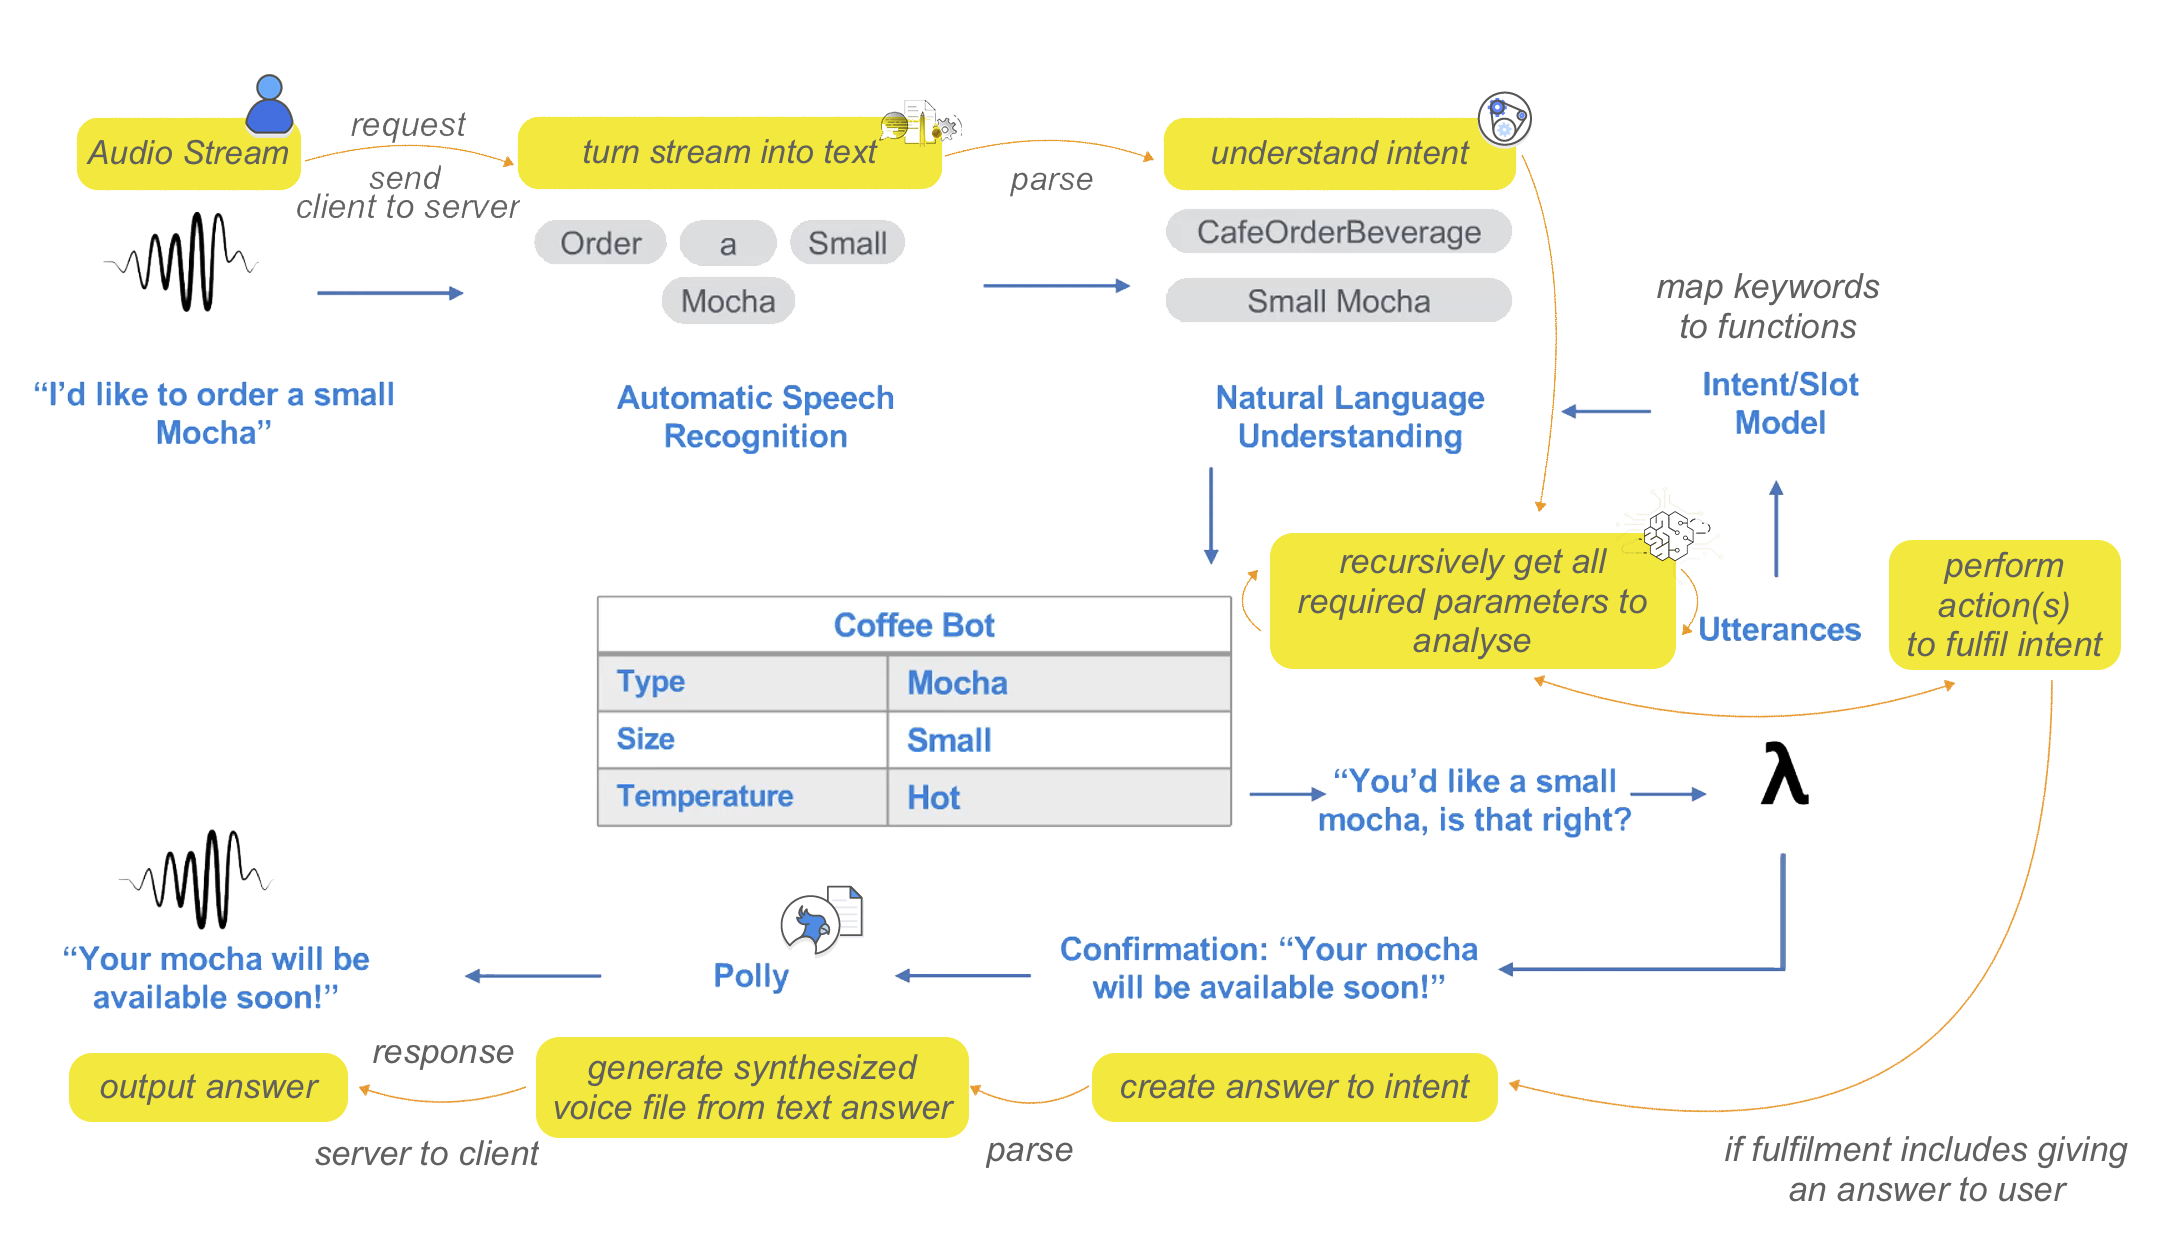
\includegraphics[width=14.8cm]{workflows/awstools.png}
\end{figure}
%
%\begin{wrapfigure}{l}{1.5cm}
%	\caption{Interaction between AWS modules in the use case of a ``Coffee Bot''}\label{lex_interactionExample}
%	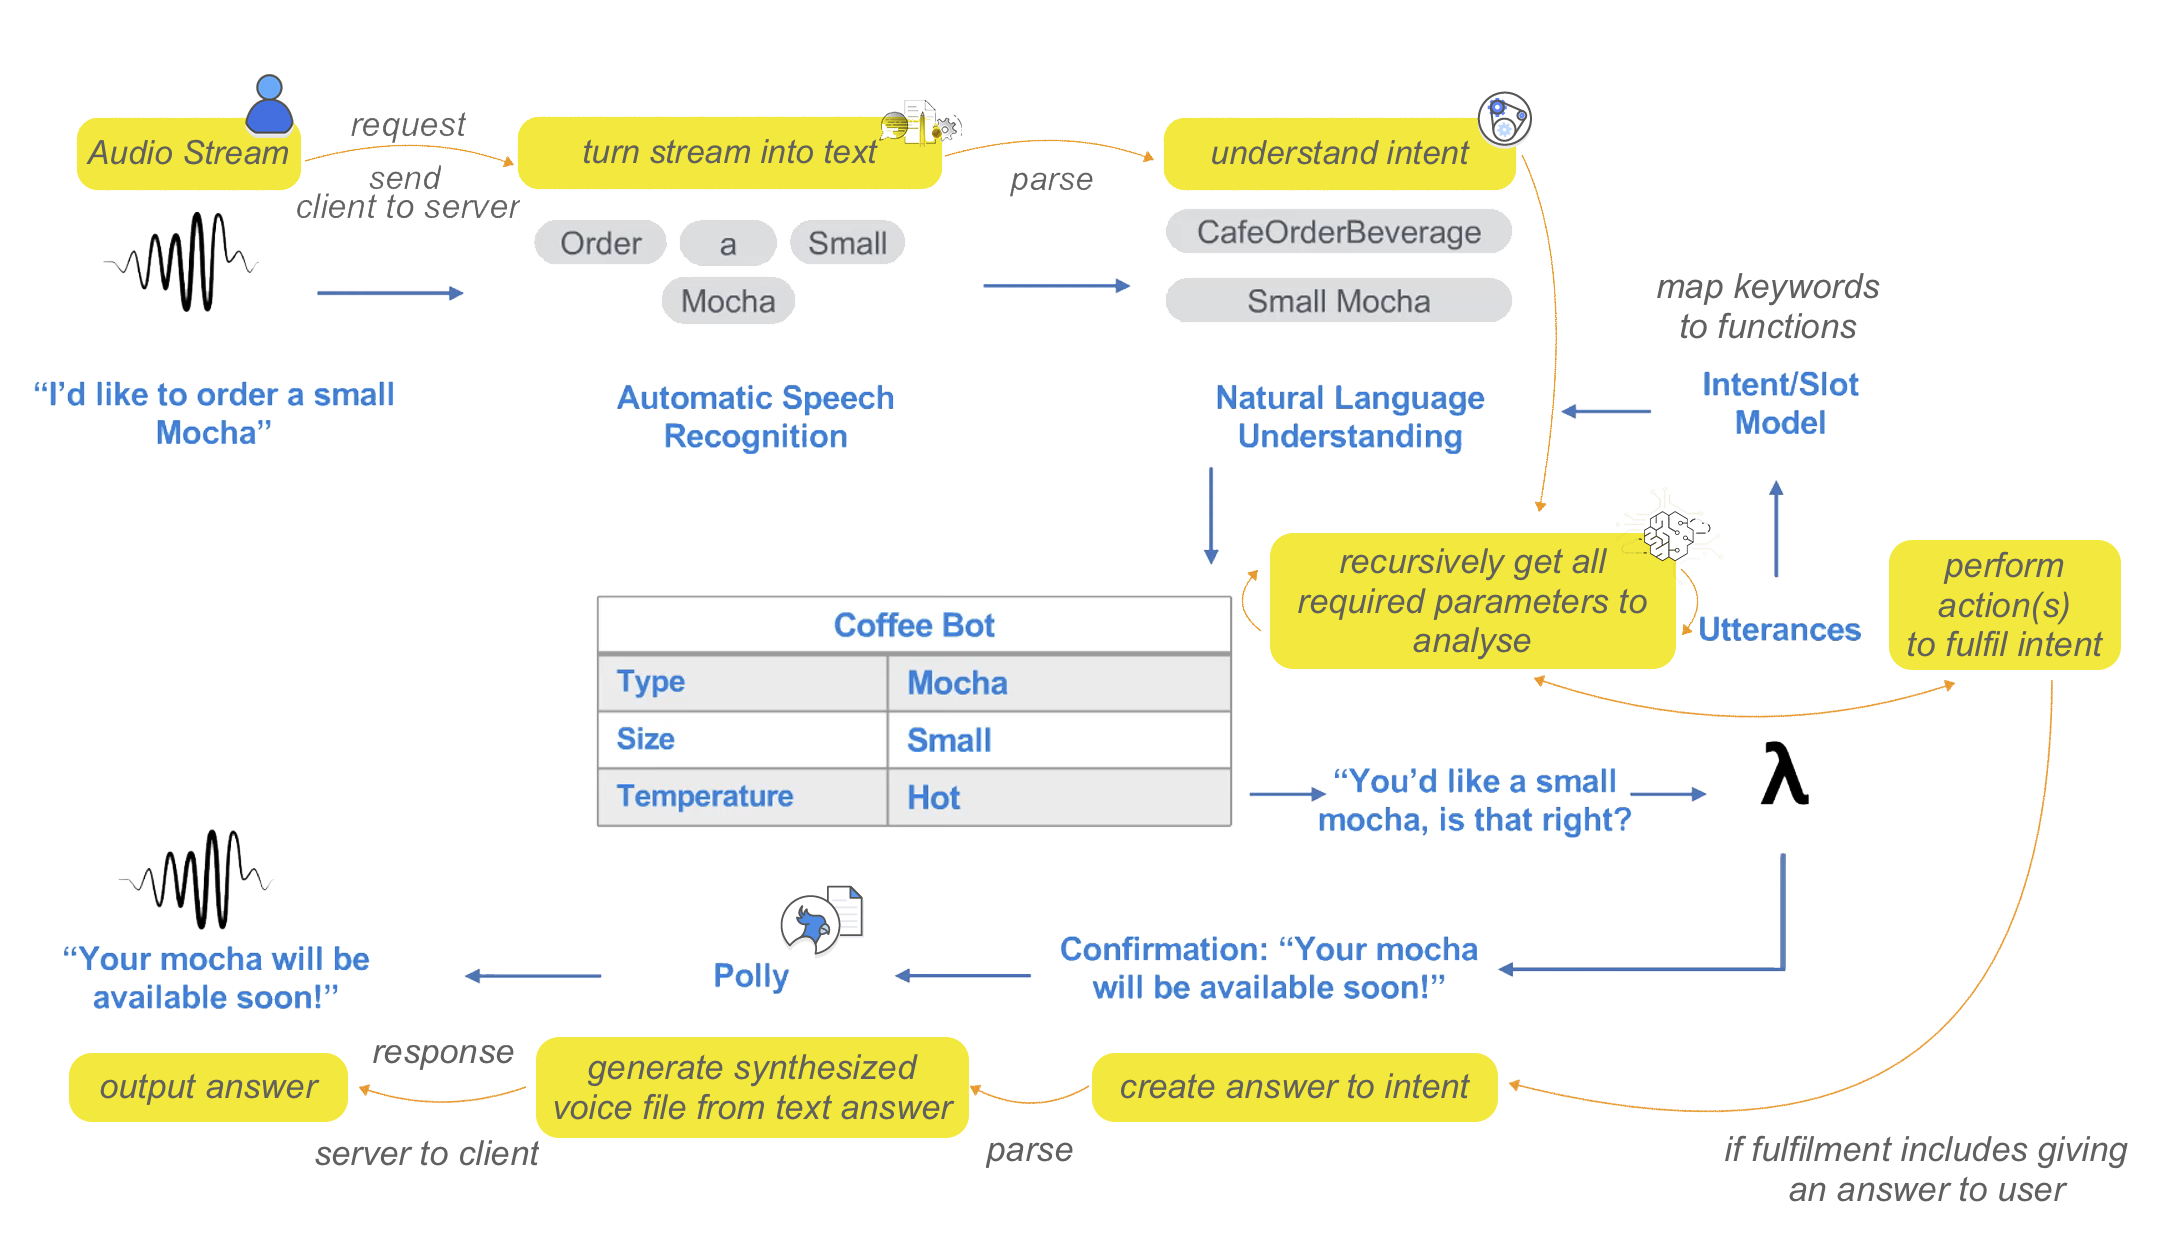
\includegraphics[width=10.5cm]{workflows/awstools.png}
%\end{wrapfigure}

putting different combinations of these and other building blocks interactively together generates the model for Alexa. In a world increasingly operated by Internet of Things (IoT), we describe a possible interaction in the example here for a use case of a hypothetical chatbot that operates a coffee machine using some of these service modules (Figure \ref{lex_interactionExample}).  Although this graphic describes how an end user would combine these modules to set up their own chatbot, this is the same workflow that Alexa uses. Hence, with Amazon's use of its own micro-services we infer that takes advantage of these to build a whole new ecosystem putting Alexa Skill developers as producers, end-users as consumers, and the Amazon website and Alexa App as a marketplace to mediate between the products (Skills) the developers produce to their target customers (end-users, country-specific or worldwide). From a marketing perspective Amazon achieves through Alexa a vertical diversification of its product programme (where existing AWS services result in a new product expanding the value chain) while simultaneously offering an extension of its aggregator model (as opposed to a marketplace model)% https://www.feedough.com/difference-marketplace-business-model-aggregator-business-model/
 by playing as a mediator between the developer's role and that of the end-user's % (who of course could be developers, too)
% this is from what I concluded from MKT and GepIT lectures.. Prof. Küpper, Axel / Prof. Klasse-Talke, Kathrin




we can therefore describe the meta-model for Alexa similar as one %to that
of an application with several front-end and back-end components acting in a DevOps environment of cloud micro-services. Unlike in most GUI-based scenarios with an MVC design pattern \cite{wiki:mvc}, where the user uses the \mintinline{java}{controller} to manipulate the \mintinline{java}{model}, which in turn updates the \mintinline{java}{view} appearing to the user, in a VUI scenario, we need to consider that the user's paradigm to the \mintinline{java}{view} component is quite different. Before we dive into the VUI paradigm, we introduce Alexa's own implementation of it for third-party applications (i.e. Skills). These are broken down into the following elements for users and developers: %to comprise a holistic ecosystem:



	
	\subsection*{Alexa Skills Store} \textit{[for End-Users]} where someone with an Alexa-enabled device can preview a Skill before installing it, %know if they want it or not and by installing them, 
	Once installed, the own instance of Alexa becomes "smarter" by that Skill, which does not need to update from ``client side'', since it is only linked to the Amazon account and not hosted on the client (only sends requests through it).  %for now 
	This offloads the user from the overhead of % does not need to 
	thinking about updates since these happen in the back-end. 
	
	
	\subsection*{Alexa Skills Kit}~\label{ask:def} \textit{[for Developers]} Although it is hard to define it as a complete SDK for Alexa and it is still in a continuous expansion phase, it is responsible for compiling the loosely coupled tools provided by AWS and others to act as an interface for the skill from a developer point of view. This fits into the rest of Amazon's scheme of focusing on interoperable micro-services that fit multiple purposes. It includes the following essentials:
	
	%Explain what the ASK SDK does
	
		\subsubsection*{Alexa (Developer) Console}~\label{ask:devconsole} This is where all the developed Skills live. It is the gateway to the front-end of the Skill or Voice service (described below). It provides a web interface for initial setup of the Skill, a structured representation of the JSON Files that include the \textsc{language (interaction) models}, the \textsc{Skill properties}, the endpoints it uses and accounts it links to. 
		Throughout this thesis, the console has undergone major interface upgrades and additions to its core functionality. Currently it is also the place where submitting the skill for publication happens and where the simulator (discussed below) lives.
		
		\subsubsection*{ASK CLI} %\lstinline|ask-cli| 
		A Command-Line Interface tool that interacts with the Alexa Console skipping the web browser. %It is still in the making but
		Although not at a stable release yet, it has numerous functions to creating, deploying and testing our Skills. %Download with 
		Available through the Node Package Manager (NPM) \footnote{
			through \mintinline{bash}{\$ npm install ask-cli} }
		
		%green because of the dollah
		
		\subsubsection*{Alexa Voice Service} %\inote{products independent from Alexa, not sure if it's worth mentioning}
		 A service for accessing cloud-based Alexa capabilities with the support of AVS APIs, hardware kits, software tools, and documentation. Through the Alexa Voice Service Amazon has simplified the creation of conversational interfaces for device makers, allowing developers to add Alexa and intelligent voice control to new products for mobile phones and cars to smart speakers and home appliances.
		 It simplifies building voice-forward products by handling complex speech recognition and natural language understanding in the cloud \footnote{\url{https://developer.amazon.com/alexa-voice-service}}


	


\section{Skill Structure}


Finally, after presenting the core stones that take part in administering the Skill, we move on to the Skill structure. Ultimately, the elements discussed above are represented in JSON files that together with the back-end of the skill make up this web-app like composition. Because of its flexible file format, Skills back-ends can be built using one of multiple runtime environments including Node.js, Java, Python, C\# and Go. 
Not coincidently, these are the same languages supported by AWS Lambda %to developed Alexa Skills. 
%can acquire access to the Skill devel

Disregarding the programming language used for development, these statically generated files are included in the code:

\begin{itemize}

\item[\mintinline{json}{skill.json}] The Skill manifest file including its publication name on the Amazon website, invocation name in each language, a description of the Skill readable by a human, author of the Skill and other properties
\inote{maybe include our sample in Appendix}

\item[\mintinline{json}{<locale>.json}] The interaction model of the respective language. It is named after the locale the file is in and includes all slots, utterances, dialogues, custom defined slot types inter alia (file structure in Table \ref{interactionModel}).

\item[\mintinline{json}{<packageFile>}] A manifest file for required dependencies (installable through NPM for instance in the case of Node or Maven in the case of Java) for installation to run the web-app in Amazon's cloud.

\end{itemize}


%\todo{remove clearpage before print}
%\clearpage

\section{Alexa Interfaces}

Briefly going over the options available to use Alexa, we present and compare the different Hardware product lines and software solutions developed by Amazon or compatible with their voice assistant in terms of usability configurations, i.e. presentation of voice and graphical interfaces.

\subsubsection*{Hardware}

The following devices are Alexa-enabled out of the box. The voice service is either accessible through voice command within the same room or an active button press on the device.

\begin{table}[htbp!]
	\caption[Alexa Devices in Comparision]{Currently Supported Alexa-Enabled Devices in Comparison}\label{alexaDeviceTable}
	\begin{tabularx}{\textwidth}{  r | l l l l  }
		
%		category
				& Speaker							& Tablet	& SmartHome	& TV	\\ \hline \hline \\
		\textit{Models}	& \shortstack[l]{Tap, Echo \\ - Dot, - Plus}     & \shortstack[l]{Echo Show \\ Kindle Fire}    & Echo Spot & FireTV Stick \\ \hline \\
		\textit{Screen}  		& No      & 7.0" 		& 2.5'' round				&  HDMI Display      \\ \hline \\
		\textit{Line Out}		& Yes      					        & \shortstack[l]{Show: Bluetooth \\ Kindle: Yes} & 	Yes & \shortstack{via HDMI \\ \textcolor{white}{text} }      \\ \hline \\
		\textit{Alexa On} 	& Voice	Command					&
		\shortstack{excl. Fire HD 10\\Button Press}
		 %\shortstack[l]{K. 7, - HD 8:  btn press \\ - HD 10: voice cmd} 
		& Voice Command & %\shortstack{Button press \\ \textcolor{white}{text} }
		Button Press
	\end{tabularx}
\end{table}

% \inote{just make a comparison table, which one has a screen, which one has which capabilities with alexa}
%Echo, Echo Dot, Tap, FireTV


%\clearpage


%then comes el software 
\subsubsection*{Software}



while the hardware models stated above are possibilities for testing, too, they do not always serve as a primary testing environment. There are sometimes more optimised ways to automate Skill testing, for instance by running scripts that would send the transcribed text in the appropriate JSON format. This is helpful for multi-turn conversations and retaining sessions, so that one does not need to repeat the full conversation until one reaches the test breakpoint.

\begin{itemize}
	
	\item[Alexa App] designed to be a control unit that operates most Alexa-enabled devices, is not an Alexa interface\footnote{yet (although this will change soon)}. However, apart from being a tool apart from Amazon's website to install Skills and manage accounts linked to Amazon (for music streaming and other related content-based services), it is a very useful tool to track the history of conversation that took place through a respective Amazon account. We use it mainly to hear what we said and see how the text was interpreted using Lex's NLU engine. It helps for checking homonyms and nuanced utterances.
	
	
	\item[EchoSim.io] ``a browser-based online community tool for developers that simulates the look and feel of an Amazon Echo'' \footnote{\url{https://echosim.io/}}. %started from a hackathon
	
	\item[Reverb] An iOS / Android app, allowing the interaction with the Alexa instance linked to an Amazon account. A perfect option to make a qualifying device alexa-enabled \footnote{\url{https://reverb.ai}}. 
	
	\item[Alexa Simulator] Alexa's own web-based online simulator giving JSON responses and voice feedback to the requests sent and is part of the ASK. We interact with it either through voice or with JSON requests. 
	
	\item[CLI Simulator] the command-line tool of the aforementioned simulator. Accepts strings and file uploads from the CLI and returns responses to the same interface. Obviously because the Skill is a web service in the cloud, the CLI also requires an internet connection \footnote{running command \mintinline{bash}{$ ask simulate --text <inputText> --locale <inputLocale>}}.
	
\end{itemize}



%%%%%%%%%%%%%%%%%%%%%%%%%%%%%%%%%%%%%%%%%%%%%%%%%%%%%%%%%%%%%%%%%%%%%%%%%%%%%



\subsection*{Speaking with Alexa}


We end this chapter by explaining how Alexa is designed to operate from the user's point of view particularly for Skills. A full guide is available in the \textsc{ASK documentation} in multiple languages. \footnote{\url{https://developer.amazon.com/docs/custom-skills/understanding-how-users-invoke-custom-skills.html}}

A conversation starts with any of the four wake words below, followed by the launch request, then the invocation name and lastly the utterance to action. Here is an example in English.:


\[
	\underbrace{\overbrace{Alexa}^{wake \  word}}_{\shortstack[r]{Computer\\Echo\\Amazon}} %Aktivierungswort
	, \ \ \ \ 
	\underbrace{\overbrace{ask}^{launch \ action}}_{\shortstack[l]{begin, launch, load\\open, play, resume\\run, start, tell, use}}
	\ \ \ 
	\underbrace{\overbrace{<my \ Skill>}^{invocation \ name}}_{\shortstack{Citizen \ Assistant \\ Georgia Gov}}
	\ \ \
	\underbrace{\overbrace{<to \ do \ something>}^{utterance}}_{\shortstack[r]{to tell me the costs of a license transfer\\how do I get my license transferred}}
\]



%###################################################################################
%###################### Topic C             ########################################
%###################################################################################











%Durchgestrichene bzw. lokalisierte/umbennante TODOs
%Done: Move node to implementation and don’t mention that you’re using lambda until In implementation chapter k

\chapter{Implementation as Alexa Skill}
\label{mainone}
%DELETEME: In this chapter you start addressing your actual problem. Therefore, it makes often sense to make a detailed problem analysis first (if not done in introduction). You should be sure about what to do and how. As writtin in the background part, it might also make sense to include complex background information or papers you are basing on in this analysis. If you are solving a software problem, you should follow the state of the art of software development which basically includes: problem analysis, design, implementation, testing, and deployment. Maintenance is often also described but I believe this will not be required for most theses. Code should be placed in the appendix unless it is solving an essential aspect of your work.

\textcolor{magenta}{
- as an example for voice\\
-System Specifications\\
-System Structure\\
-UML Diagrams\\
-Design Choices\\
-scopes and granularity
}

\section{All about Alexa}
\url{https://en.wikipedia.org/wiki/Amazon_Alexa}
\url{https://medium.com/@robinjewsbury/how-to-create-bots-and-skills-for-facebook-messenger-and-amazon-echo-4a03935eeca1}
\textcolor{magenta}{
- Alexa Appstore had over 5,000 functions ("skills") available for users to download,[18] up from 1,000 functions in June 2016.
}
\textcolor{red}{McLaughlin, Kevin (16 November 2016). "Bezos Ordered Alexa App Push"Paid subscription required. The Information. Retrieved 20 November 2016.}

\textcolor{red}{Perez, Sarah (3 June 2016). "Amazon Alexa now has over 1,000 Functions, up from 135 in January". TechCrunch. Retrieved 5 August 2016.}

\section{Difference Between Lex and Alexa Skills}  
\url{https://stackoverflow.com/questions/42982159/differences-between-using-lex-and-alexa#URL}\\
\url{https://aws.amazon.com/lex/faqs/}\\
\url{https://aws.amazon.com/about-aws/whats-new/2017/09/export-your-amazon-lex-chatbot-to-the-alexa-skills-kit/}\\
\textcolor{magenta}{Amazon Lex is a service for building conversational interfaces using voice and text. Powered by the same conversational engine as Alexa, Amazon Lex provides high quality speech recognition and language understanding capabilities, enabling addition of sophisticated, natural language \'chatbots\' to new and existing applications. Amazon Lex reduces multi-platform development effort, allowing you to easily publish your speech or text chatbots to mobile devices and multiple chat services, like Facebook Messenger, Slack, Kik, or Twilio SMS. Native interoperability with AWS Lambda, AWS MobileHub and Amazon CloudWatch and easy integration with many other services on the AWS platform including Amazon Cognito, and Amazon DynamoDB makes bot development effortless.}


\section{APIs and SDKs}

\textcolor{magenta}{
- swagger for handling JSON requests?\\
- \url{https://github.com/alexa/alexa-skills-kit-sdk-for-nodejs}
}

\section{challenges}

\textcolor{magenta}{
- und L\"osungen daf\"ur\\
- eine \"Uberf\"uhrung in Alexa, not writing everything new in alexa. such that when you want to do it in another system what do u want to integrate?\\
- use external web service maybe? in case that helps instead of alexa doing everything..\\
- konten hosting to be on alexa\\
- wo hilft mir alexa, was mach ich lieber woanders?\\
- \"Ahnlichkeitsma{\ss}e -levenstein-distanz, IFTTT
}
\chapter{Skill Implementation}%: \inote{Kosten-/Terminabfrage}}
\label{maintwo}

In this chapter we present our implementation solution through the code provided. %and hands-on experience throughout.
%The code 
%available 
In addition, the project on Github (see Chapter \ref{introduction}) is expected to be maintained %with plans for development 
beyond the scope of this thesis. A copy is attached to this work, but cannot fully operate as a standalone software given the dependencies it has to Alexa's SDK described in previous chapters. The runtime environment is offered through the ASK. %\inote{github, the new amazon account? ...}
There are many ways to %perform setup
set up the project, several languages we can use to programme 
our Skill (Chapter \ref{mainone}) and throughout the development process some of these steps were altered from Amazon's side. %changed. 
As mentioned, we settle for the most recent interfaces and implementation possibility using Node.js hosted on AWS Lambda. %, However, this is very likely to change in a near future.

\section{Setup}


%\todo{codechunks different labeling??
%}

\subsection*{Minimum Requirements}
For the environment setup, the following tools and credentials are necessary:

\subsubsection*{Amazon Account}
We use it in conjunction with AWS and the Alexa Developer Console. Any account previously created for the Amazon store is usable \footnote{e.g. from here  \url{https://aws.amazon.com/de/resources/create-account/}} as well as to test our Skill. Once the account is activated on the developer console, the Skills in development become automatically reachable on any Alexa-enabled device linked to the same account (as an end-user). Their invocation names also precede those of installed Skills. If two Skills in development have the same invocation name, the first registered one will be invoked.
	
\subsubsection*{Command Line Tools}
\begin{itemize}
\itemsep0em
\item \textbf{Python 3} or\textbf{ Ruby 4} need to be installed as a foundation for ASK CLI and AWS CLI.
\item  A package manager such as Pip Installs Packages (\textbf{PIP}) for Python or \textbf{RubyGems} for Ruby.
\item  Depending on OS, further packages and package managers might need to be installed. (e.g. for macOS: Command-Line Tools for Xcode, Homebrew, easyinstall). These will be prompted throughout the installation process.
%\inote{brew, easyinstall python / win}

\end{itemize}

	
\subsubsection*{API} 
As introduced in Section \ref{Solr}, Our endpoint is a Solr Server that provides us with JSON responses to the queries we do through a RESTful interface from within the Lambda function (hosting back-end code) \footnote{reachable at the time of development on:\\\url{https://newsreel-edu.aot.tu-berlin.de/solr}}. Since the API endpoint was originally created for the Virtual Citizen Assistant, we need to readjust its output to meet Alexa's requirements and host a second instance of it to make it reachable not only locally, but also for Lambda. The containing server is secured with SSL to meet with AWS's encryption standards.

%
%\todo{
%Technology:	Lucene
%spell check. unscharfe suche
%…Tika / detect language / … it’s the golden standard
%Solr
%Data Structure: XML datei, (hierarchical)
%
%}




	
\subsubsection*{Audio} An encoder to create 48kpbs constant bitrate MP3-Format. Audacity \footnote{\url{http://www.audacityteam.org/}} or FFmpeg\footnote{convert by running \lstinline|$ ffmpeg -i <inFile> -ac 2 -codec:a libmp3lame -b:a 48k -ar 16000 <outFile.mp3>|} can be used to convert to an Alexa-friendly file format like in the \textsc{ASK Documentation}\footnote{\url{https://developer.amazon.com/de/docs/custom-skills/speech-synthesis-markup-language-ssml-reference.html\#h3_converting_mp3}}.
	


\subsection*{Managing AWS Credentials}

With the Amazon account we just created (or already acquired), we proceed to extend it for developer use by registering with AWS. %registration. 
As we move within the free tier of AWS, no charges were applied. A credit card might be required for eventual future billings if the tier limitations were exceeded. We mention pricing schemes in Section \ref{devmodels}. More information on pricing available on AWS \footnote{\url{https://aws.amazon.com/de/pricing/}}. Developer registration needs to happen on AWS website\footnote{\url{http://aws.amazon.com}} as well as on the Amazon Developer Portal\footnote{\url{https://developer.amazon.com}} separately, where some additional information is required such as company name and business sector. A vendor ID required for use with Amazon is generated. From this point on, any code that manages the back-end of our skill will be associated with AWS Modules, primarily Lambda. Skill configuration and interaction model are hosted on Alexa Skills Kit separately, i.e. managed through the Amazon Developer Console. During the development process, Alexa Skills Kit diverged from the Amazon Developer Console and has become a separate entity called Alexa Console. While still hierarchically belonging to the Amazon Developer Console and reachable from the same domain, except for the developer profile, all Skill-related information we need to use are modifiable from within the Alexa Console\footnote{\url{https://developer.amazon.com/alexa-skills-kit}}. The separation from Lambda also means that code we need from the interaction model has to be duplicated from the Skill, since Lambda does not have access to Alexa Skill and can only be used as a trigger

\subsubsection*{Generating Access Keys}~\label{accesskeys}
Linking happens through a private and public key pair - the \textbf{access keys} consisting of a
combination of an \textit{access key ID} (like \lstinline|AK..7EXAMPLE|) and a \textit{secret access key} (e.g \lstinline|{wJalrXUt..I/K7..G/bPx..YEXAMPLEKEY|). We use access keys to sign API requests made to AWS.

Creating Access Keys is described in the \textsc{AWS Documentation}\footnote{\href{https://docs.aws.amazon.com/general/latest/gr/managing-aws-access-keys.html}{\t{a\t{ws}}/\lstinline|/latest/gr/managing-aws-access-keys.html|}}. At this time we interact with the IAM Module from AWS (Identity Access Management) implicitly, which defines roles of each member in an organisation and partners linked to it, who can gain different levels of access to each module capabilities. Since we are only making basic use of AWS modules and our Lambda instance interacts only with our own API, there is no harm in using 


\subsection*{Initialising The Development Environment}

As minimum package requirements can vary a lot between one OS and another, using a virtual machine is suggested for teams. AWS offers Elastic Compute Cloud (EC2) as a service for virtual machines in the cloud. Although this step is mainly for performing command-line prompts later on, %if opting for that, 
with this option it is convenient to avail a web browser inside the virtual machine instance. Otherwise, for browser communication %the tool we are using
AWS CLI generates URLs with the \mintinline{bash}{--no-browser} parameter that we %would need to copy and 
paste into a browser outside of the virtual machine to link it with the Amazon account we use.

%Once 

\subsubsection*{Creating Lambda Instance}

Although the ASK CLI makes it easy to perform multiple setup steps at once, at the time of this project, this option was not available. Having started with an AWS account in North Virginia as a server region as the only available server that accepts Alexa Skills as a trigger for Lambda, changing the server location to Ireland was complex in the sense that both servers are completely separated from one another \footnote{
%my link to Amazon Developer Forums
\url{https://forums.developer.amazon.com/questions/87860/ask-cli-eu-lambda-region.html?childToView=164883\#answer-164883}}.
Hence the migration had to be done manually. Additionally, all CloudWatch logs are not transferable between regions. At the time of completion of this project, the AWS server based in Ireland (\mintinline{java}{eu-west-1}) % writing this th
was the most preferable for latency. Moreover, as this project ends before AWS's terms were readjusted to accomodate with the GDPR, hosting on the Ireland server implied different regulations about code ownership and accessibility.

Once a Lambda function is ready to be created, we assign it the role \mintinline{java}{lambda_Execution_basic} then link the trigger as an Alexa Skill.

To make sure the Lambda instance is not invoked from nowhere else, we tie it to the Skill's resouce number in the trigger configuration.

Verification through Application ID is described in the \textsc{ASK Documentation} \footnote{\href{https://developer.amazon.com/docs/custom-skills/handle-requests-sent-by-alexa.html\#request-verify}{\t{a\t{sk}}\lstinline|/handle-requests-sent-by-alexa.html\#request-verify|}}


%
%\todo{creating lambda alone}
%
%
%\todo{cmd --no-browser\\
%	setting up lambda alone not based on skill, since we want to use Ireland not US. so we create a new function and give it the IAM role
%	
%}


\subsection*{Installing Command-Line Tools}
This script % offers an orientation on the configuration
checks if resouces are available then installs the AWS and ASK CLIs.

\begin{minted}[linenos,tabsize=2, bgcolor=bgkolor, breaklines, fontsize=\footnotesize]{bash}
	$ which node			#check if installed
	$ which npm			 #check if installed
	$ which python		#check if installed
	$ which ruby			#check if installed if proceeding with rbenv
	$ python --version #we use 3.5.3
	$ node --version	 #we use 7.3.0
	$ npm --version 	 #we use 4.1.1
	$ pip install aws-cli #Amazon Web Services Command Line Interface
	$ aws --version		#check successful installation. We use aws-cli/1.15.1 Python/3.5.2 Darwin/15.6.0 botocore/1.10.1
	$ npm install ask-cli| #Alexa Skills Cit Command Line Interface
	$ ask --version	  #we use 1.1.6
\end{minted}


\textsc{AWS documentation} \footnote{\href{https://docs.aws.amazon.com/cli/latest/userguide/cli-chap-getting-started.html}{\t{a\t{ws}}/\lstinline|cli-chap-getting-started.html|}} provides more information on special configurations

%\begin{minted}[linenos,tabsize=2,breaklines]{bash}




\subsection*{Understanding the API Query parameters}
%HTTP(S) endpoint:
%\url{http://newsreel-edu.aot.tu-berlin.de/solr/#/d115}
Solr cores are accessible with the respective core name appended to the base URL.
%Rest Query
%Solr Syntax (only url. he knows solr better than i do)
Query syntax can be passed as parameters in the URL, too, like in the following example.



\url{https://newsreel-edu.aot.tu-berlin.de/solr/d115/select?q=ladenoeffnung*&wt=json&indent=true}
\begin{enumerate}
	\itemsep0em
	\item \textbf{Credentials: } \mintinline{text}{username:password@}
	\item \textbf{Base URL:} \mintinline{text}{newsreel-edu.aot.tu-berlin.de/solr}
	\item  \textbf{Path:}	
	\begin{itemize}
		\itemsep0em
		\item Core: \mintinline{text}{d115}
		\item Query: \mintinline{javascript}{/select?q=} QueryText
		\begin{itemize}
\itemsep0em
			\item Query Parameters: we can use usual Solr parameters in the API Calls (e.g. wildcards (*), concatenation (+), AND operator) \footnote{Available Syntax: \url{http://www.solrtutorial.com/solr-query-syntax.html}}.
			\item MIME Type: \mintinline{text}{&wt=json}
			\item Other Parameters: e.g. \mintinline{text}{&indent=true}
					\end{itemize}
		
	\end{itemize}
	
\end{enumerate}



%
%
%
%
%step by step code analysis
%
%\url{https://github.com/alexa/alexa-skills-kit-sdk-for-nodejs/blob/master/Readme.md}
%



%\subsection*{requirements}
%
%for audio (old)
%
%json format https://stackoverflow.com/questions/41776014/how-to-correctly-specify-ssml-in-an-alexa-skill-lambda-function




%
%references:
%
%\url{https://developer.amazon.com/docs/custom-skills/speech-synthesis-markup-language-ssml-reference.html#audio}



%blogs:
%\url{https://developer.amazon.com/post/Tx3FXYSTHS579WO/Announcing-New-Alexa-Skills-Kit-ASK-Features-SSML-Audio-Tags-and-Developer-Porta}

%With the JSON we have, we try to maximise its use, but we need to consider that with starting a Skill, it is better to start from scratch sometimes and as we go, we see what is the relevant information that we can integrate into our Skill.
%
%We analyze the output of the \textsc{Virtual Citizen Assistant } and realize it makes less sense to start with that, so we refer to the underlying endpoint. Since this is the Solr Server that delivers JSON objects and is more realistic to maneuver, we analyse the queries we can get from there. and try to fit it into our interaction model.
%
%Then we move on to the interaction model. On paper, we draft the use-cases to determine what are our intents first to group these into fewer intents than the services we have. Given that there are many public services related to a similar case, we design our Skill to make it possible to group them into less intents. The advantage of this is that it allows us to at least have fewer 'ServiceIntents' than the ever growing number of services, which means that we want to also be able to track new services as they get inserted into the catalogue to be able to either map them to old intents by extending these, or to introduce new intents if this does not work.
%
%
%
%\todo{ moved from intro\\
%
%
%our now more than \inote{4}
%scenarios:
%\begin{itemize}
%	\item a general scenario of predefined categories related to any service \tocite{hier schon erwähnen? \inote{(prerequisites, costs, documents, ...)}}
%	\item special application on \textbf{Residence Registration} - ``Anmeldung einer Wohnung''
%	\item special application on \textbf{Applying for a Residence Permit} - mutliple services related to ``Aufenthaltstitel''
%	\item ``car registration'' -  special application on \textbf{Car Registration''} - multiple services  related to ``Kraftfahrzeug (KFZ)''
%	%	\item[scenario 4] \inote{yet to be decided or if to implement}
%\end{itemize}}
%
%%%%%%%%%%%%%%%%
%
%
%
%\todo{moved from AWS Micro-services list\\
%
%	We might as well use just our own, any other privately or cloud-based server solution to host our code and use it as an endpoint for our software, however choosing Lambda takes away the overhead of linking the front-end with the back-end of the Skill %program we develop (an Alexa Skill as we describe below). 
%
%}
%
%%%%%%%%%%%%
%
%
%
%
%
%
%%\section{step-by-step}
%
%start with interaction model
%then use builder
%then fulfill functions
%
%
%steps to git commit
%deploy
%clone
%change in browser
%change offline


%if u use a browser, remember to keep the session active otherwise your model might get lost in the POST









%\todo{this goes after we have a lambda instance connected to our skill}








%\section{Code Analysis}


\subsection*{Event Emitters}

In all Intent handlers, a common pattern is to generate speech output from Alexa with a certain result or question, then allow the user to speak or end the session as discussed in Section \ref{sessionduration}.


As per description in Section \ref{nodejs:def} A \mintinline{java}{LaunchRequest} always starts a new session. Event Emitters can be categorised in the following Table \ref{evtemit}. 
``The difference between \mintinline{text}{:ask/listen} and \mintinline{text}{:tell/speak} is that after a \mintinline{text}{:tell/speak} action, the session is ended without waiting for the user to provide more input'' \footnote{\href{https://github.com/alexa/alexa-skills-kit-sdk-for-nodejs/blob/master/Readme.md}{\t{gh}/\lstinline|alexa-skills-kit-sdk-for-nodejs/blob/master/Readme.md|}}. %We will compare the two ways using response or using responseBuilder to create the response object in next section.

\begin{table}[H]
	\caption{Event Emitters}
	\label{evtemit}
	\begin{tabu} to \linewidth {X[2] | X  X[3]| X[3]}
Emitter Type & \multicolumn2{|c|}{Emitter Name} & Session Ends\\ \hline \hline

\shortstack[l]{Speech Out \\ (only Alexa)} & \mintinline{text}{tell} & \shortstack[l]{ \mintinline{text}{speak} \\  \mintinline{text}{:responseready} } & \shortstack[l]{\mintinline{java}{true}\\(no wait for response)}\\ \hline

\shortstack[l]{Speech Out / \\Recording} &  \mintinline{text}{ask} & \shortstack[l]{ \mintinline{text}{listen} \\  \mintinline{text}{:responseready} } & \shortstack[l]{\mintinline{java}{false}\\(conversation continues)}\\

	\end{tabu}
\end{table}

Effectively, an emitter sends a response to a JSON request (example in Appendix \ref{jsonFromAlexa}) with parameters that determine whether the session remains on or no, what the response includes and a device token to direct the response to the right Alexa-enabled device.





%jsons sent/received in appendix














%\section{Code Analysis}
\section[Features]{Feature Implementations}



\subsection*{Intent Implementation}
\textit{e.g. index.js \quad : \quad  DE\_handlers \quad :  \quad AMAZON.HelpIntent}\\
% Wi, certain intents have to be added and fulfilled (HELP, STOP, …)
As the actions resulting from \mintinline{java}{HelpIntent, StopIntent} and \mintinline{java}{CancelIntent}
have to be decided on, we choose to make the \mintinline{java}{HelpIntent} for non-contextual help, giving the contextual help as a prompt inside each intent separately.
The \mintinline{java}{StopIntent} terminates the Skill and the \mintinline{java}{CancelIntent} ask to restart to a new intent within the Skill.


\subsubsection*{Making the right conversation}
In certain intents like with a question about residence permit for non-EU residents, there is a pattern of questions to be asked in a given order as a public official would do. This is related to the law structure, given than certain regulations have precedence over others. In this example, the EU-partner rule is applicable, where EU laws supersedes local regulations.
As such, if a non-EU/EEA resident wants to apply for a residence permit for any purpose and have an EU-partner (swiss regulations similar but have a different legal base), the residence purpose should be the Freedom of movement of an EU-citizen and their family and not the other reason the person is applying with.
%legal things like the EU-partner rule.
How EU rules override local ones is codified in
% bas u cant explain it to people 3ashan they have to be give the choice.
el mawdou3 mo3aqqad but codified in Directive 2004/38/EC \footnote{
\url{https://eur-lex.europa.eu/legal-content/EN/TXT/?uri=CELEX:02004L0038-20110616}}.



\subsection*{Dialogue Management}
As we explained dialogue directives in Section \ref{directives:def}, we use them in our code to delegate a few responses to the interaction model \footnote{ \t{a\t{sk}}\href{https://developer.amazon.com/docs/custom-skills/dialog-interface-reference.html\#delegate}{\lstinline|/dialog-interface-reference.html\#delegate|}	
}


\subsubsection*{Guessing the right Location}
\textit{e.g. index.js \quad : \quad  DE\_handlers \quad :  \quad LOC\_WhereIsAreaOrPLZ\_Intent}\\
One of the Intents answers the question where a certain PLZ or district is in Berlin. It does not use geocoordinates but is sensitive to nuances in uttering a PLZ, as these are not always pronounced as individual digits but sometimes as a combination between a number and digits. For instance, in German we say ``Zehn Eins Eins Neun'' for 10119, which is a code belonging to two different districts. Alexa is able to determine this through elicitation as well as dealing with some special cases like when the number is outside of Berlin.





\subsection*{Randomising Alexa's Utterances}
\textit{e.g. ./lib/helper.js \quad : \quad  \mintinline{text}{randomphrase()}} \\
With word arrays, we are able to generate a random answer, such that every time the user expects a different answer from Alexa, simulating a natural conversation. %What’s next doesn’t look what came before



\subsection*{Creating SSML and Audio}
\textit{e.g. index.js \quad : \quad  DE\_handlers \quad :  \quad LaunchRequest}\\
Used to generate sound effects during the conversation such as emphasising certain words or whispering and playing short audio clips \footnote{\href{https://developer.amazon.com/docs/custom-skills/speech-synthesis-markup-language-ssml-reference.html\#audio}{\t{a\t{sk}}\lstinline|/speech-synthesis-markup-language-ssml-reference.html\#audio|}}.







\subsection*{Checking the Next available appointment}

With this work as a proof of concept, and an API extension from ITDZ's side, it is equally easy to implement a feature to look up next available appointments.
The actual booking would require Alexa to send POST requests and persistently retain these on the API's side with the option to impement another feature to save the same appointment to the calendar linked to the Amazon account used with this Alexa instance. This might require account linking, too, if we need to pass the appointment data through the Skill to an online personal calendar endpoint, bypassing Alexa itself.

Booking an appointment happens for now only through Berlin.de's website by starting at either \href{https://service.berlin.de/terminvereinbarung/termin/}{the appointment booking page} \footnote{\url{https://service.berlin.de/terminvereinbarung/termin/}} which links to the actual booking pages via choosing the service or the location where the service 



\subsection*{Card Templates}

%Rendering the right template or a custome one
We can render a different template for each device type. For our purpose, the standard template is sufficient. Customisation can be useful with displaying longer texts. \footnote{\href{https://developer.amazon.com/docs/custom-skills/display-interface-reference.html}{\t{gh}/\mintinline{java}{display-interface-reference.html}}}

%
%\todo
%unhandled always calls or never


\section{Testing and Deployment}

continuous testing during development is vital before evaluating the system as a whole. % during development, noch nicht evaulation, although the same techniques are pretty much used afterwards. Requires 10 users a day to generate
With the testing tools introduced in Section \ref{testdevices}, it is important to test not only every feature indiviually, but also in combination with other features already implemented.



The more complex the Skill gets, the more important to make error handling integrate in the code. Excessive logging does not affect the skill performance per se, as the user does not see the console logs. % is  good practice. % not bad as long as it does not get too confusing.
All logs are visible on CloudWatch, with the ability to set alarms if certain warning levels were reached. CloudWatch logs can also show why some intents are never reached.



%Postman

%\todo{history API - Dave isbitzkis tweet}
The Skill Management API provides short commands to check the intent history  \footnote{\$ \mintinline{bash}{ask api intent-requests-history <--skill-id <skillId>>}\\ \mintinline{text}{[--filters <value>] [--max-results <value>] [--sort-direction <value>] }
\mintinline{text}{[--sort-field <value>] [--next-token <value>]}\\


\url{https://developer.amazon.com/docs/smapi/ask-cli-command-reference.html\#intent-requests-history-subcommand} and \\ \url{https://developer.amazon.com/docs/smapi/intent-request-history.html}
}





For most test, deployment is needed.
We deploy eiher the whole Skill or in parts, depending on where we implement a new feature

\begin{minted}[tabsize=2, bgcolor=bgkolor, breaklines, fontsize=\footnotesize]{bash}

ask deploy -t|--target lambda
\end{minted}

deploys only the lambda function, shortening the time required for rebuilding the interaction model.
%\section{Deployment}

Once a Skill is ready for publishing, it can proceed to approval, 
	%Continuous Skill 
%approval is 
the process of Amazon deciding whether each uploaded version / update is still fit for purpose, make the skill better or worse in conjunction with other skills on the Store % or change things to worse partly





%Solr is not secure (ein kleines thing in future work)
%Solr has to be secure
%\url{https://docs.aws.amazon.com/AmazonS3/latest/dev/WebsiteEndpoints.html#WebsiteRestEndpointDiff}

%
%Hey:
%
%do this set up as prerequisites first
%as a deployment script
%
%- install aws cli
%- install ask cli
%- set up a profile on AWS
%- ask init etc.


%
%There is no AWS credential setup yet, do you want to continue the initialization?
%
%https://developer.amazon.com/docs/smapi/quick-start-alexa-skills-kit-command-line-interface.html



























%Manage IAM roles (User, groups, rights, policies etc.)


%all logs go onto cloudwatch
%including when the request is not right etc...can be helpful to know what users want, beyond testing





%amazon does not disclose avaliable values for their slot types (lists), but they give you examples here
%%https://developer.amazon.com/docs/custom-skills/slot-type-reference.html#h2_extend_types


%===

%finally, we had to resolve to the information publicly available to tailor custom scenarios


%-====inserted



\section{Challenges}
\label{challenges:design}



Throughout the implementation process, many challenges were faced with respect to the runtime environment and the constant changes from Amazon.
In the following are some of the encountered  obstacles.

\subsection*{Interaction Model}
Building the interaction model on the web is a long process. %could take a long time. 
As login sessions need to be refreshed, once a session is expired, changes in the model in the browser can get lost. This was fixed by receiving a warning once trying to save the model only recently.
It can also get confusing to deploy from two different locations (CLI and web browser) without knowing which is the most up-to-date. 
% can Sessions were not active and changes were gone but amazon fixed that later giving a warning message

\subsection*{Interpolation from Virtual Citizen Assistant}
%first one: we start of with finding a way to interpoloate our model
%direkte übernahme ist nicht möglich, da die nodes nicht einheitlich geparsed werden kuönnen (fees etc)
Finding a solution to map the structure of the Virtual Citizen Assistant is not straightforward as there exists little documentation resources for the programme.
%- I also do not have any documentation of the current bot
Also, with the data in the API not coherent (e.g. Fees do not have the same data type and structure), makes it not an immediate takeover.

\subsection*{Environment}
%- problem is: if i use screenshots and amazon changes the interface (in the process)
%As the developer console changed interfaces
As many interfaces were changed by Amazon, knowing how to operate the new interface requires an extra amount of time to relearn the new functions and their locations.

\subsection*{Transcription}
With only some of the concepts of Alexa's methodology known, the software is a black box and not predictable. How Alexa's NLU engine transcribes a user's voice can become problematic with long constructed words. In German, `Hohenschönhausen' or `hohen schön hausen' is one such examples.


%\textcolor{magenta}{
%	- und L\"osungen daf\"ur\\
%	- eine \"Uberf\"uhrung in Alexa, not writing everything new in alexa. such that when you want to do it in another system what do u want to integrate?\\
%	- use external web service maybe? in case that helps instead of alexa doing everything..\\
%	- konten hosting to be on alexa\\
%	- \"Ahnlichkeitsma{\ss}e -levenstein-distanz, IFTTT
%}

%ending an utterance with a Fragezeichen
%Error: There was a problem with your request: ``werden?'' in the sample utterance ``TestIntent was soll aus dieser Skill werden?'' is invalid. Sample utterances can consist of only unicode characters, spaces, periods for abbreviations, underscores, possessive apostrophes, and hyphens.
%
%do not use "?"

\subsection*{Provided Data}
problems with countrylist
cote d'ivoir, südsee (british territories overseas, ...)




% ===
% mentioned in prev. chap but not as challenge
%once you upload the new lambda, the old one is gone, unless you version it like this:
%https://docs.aws.amazon.com/lambda/latest/dg/versioning-aliases.html
%
%
%
%====

\subsection*{Outdated Resources}
Online resources are rich but are not always up-to-date. %While it's hard for a beginner with no knowledge of the current status of
With new features from Amazon launched almost weekly, keeping with the trend requires a dedicated amount of time.
While outdated resources are not relevant for development, they can provide a good understand on how a Skill operates. %the best 
%
%first i got screwed over with this Big nerd ranch then this happened: alexa-skill module
%- so don't use this tutorial, although very helpful for a beginner and makes you understand what happens under the hood, it has been abstracted in many other function and the logic is no longer the same. - which explains why no one starred it
%
%https://github.com/matt-kruse/alexa-app
%
%https://www.bignerdranch.com/blog/developing-alexa-skills-locally-with-nodejs-deploying-your-skill-to-staging/

%
%
%\todo{
%	OnLaunch\\
%	IntentHandler\\
%	intent is triggered by utterence\\
%	account verlinkungen etc\\
%}
%
%Prob with outdated tutorials
%
%\todo{
%eventually mention here: \\
%as we mentioned Amazon's strong take on constant changes, we will go over the workarounds and circumventions to retain a working version of the Skill we present, discuss the downside of adaptability to these changes \inote{(constantly basastem nafsi 3ala 7aga gedida)}
%}



\section{Summary}

In short, the development of a Skill for an E-Government solution is feasible with the aforementioned considerations. The submitted code is a viable product which can be used for further development to produce a useful Skill to Alexa user in Berlin. With this example, similiar implementations can be done for other cities of the same information capacity.



\chapter{Evaluation}
\label{evaluation}
%DELETEME: The evaluation chapter is one of the most important chapters of your work. Here, you will prove usability/efficiency of your approach by presenting and interpreting your results. You should discuss your results and interprete them, if possible. Drawing conclusions on the results will be one important point that your estimators will refer to when grading your work.



\section{WienBot}

\todo{
-versteht nicht, wenn ich `perso' schreibe\\
-verbose.. "warum möchten Sie aus der Stadt...\\
-uses emojis\\
-speech recognition happens on device (iOS)\\
-use failed attempts of screenshots (new and old)

}
\section{GeorgiaGov}


child care
vs child custody. Sorry i didnt get that. (check first skizze)

\begin{figure}[p]

	\caption[Conversation Flow on Georgia.gov]{Activity Diagram of Conversation Flow on Georgia.gov}
	\centering
	\includegraphics[ height=\textheight]{Georgia2}
	\label{astah:georgiaActivity}
\end{figure}

\todo{
-This is how their model works:\\
services are grouped into categories as seen on \href{http://www.georgia.gov}{georgia.gov}\\
-Alexa catches from any sentence you say only the service grouping name.\\
-then gives you a definition\\
-then asks you if you want to hear about related services (in the format of FAQ)\\
-possible examples: ``I am 17 and my parents are blind. How do I renew my license?''\\
-it goes through this list and you can say yes and no if you want to hear about the `related' item.\\
-of the related items are questions like `how much does it cost', `how much time does it take'. These are no explicitly put in the questions you can ask but they become clear if you have time to make conversation. (Kritikpunkt!)
-then when it reaches the end of the list it says that it's over and if you want to have the phone number that is related tot this service grouping
%
%
%
-then the conversastion either ends or restarts.\\
-you can ask questions only about service groupings\\
%
%
-stop and cancel intent:
\textit{Feel free to ask another question or say exit}
-helpIntent:
Ask me a question
%
repeat does
%
-reprompts are not very ueful and repetitive
}


This way, if a user does not see this service is relevant to them, they will say no and skip to the next

\section{Alexa in General}
Experian of Alexa as a whole \url{https://www.experian.com/innovation/thought-leadership/amazon-echo-consumer-survey.jsp}


\todo{are Skills really going to make it?
	
	30,000 users a day in the US
	\url{https://omr.com/en/amazon-alexa-skill-marketing/}
	10,000 BVG

}


\todo{sometimes voice will hardly or never get what you want. try to tell alexa to play YAS. will always redirect you to something else}


\todo{- wo hilft mir alexa, was mach ich lieber woanders?\\
	- wie kann man die G\"ute des Systems beurteilen? \textbf{do not forget the surveyu made}   }

\section{Metrics}

\todo{
\textbf{talk about umfrage-design:}\\
skalen, yes no, choosing between limited answers, etc.\\
combining logic and validation, such that you would be asked about only one thing if you answered the other respectively.
done in english and german for purpse: cater for different people living in berlin\\
conjoint analyse\\
a-b testing - see what users prefer then come to conclusion that dienstleistung is the most important\\
we evaluate how people speak to alexa with sample sentences.\\
ask questions like "Did u know berlin.de has a behindertenberechtigt" to educate the person at the same time\\
}

\todo{
what disturbs you  most about alexa?\\
would u try it again if the question fails?\\
-thats why the retention rate is low
}
\todo{
NPR\\
time series
a-b testing
weighting
use of correlations in the legal system (got, defaulting)
search map predicts ur personality
fear of judging, fear,…interdependence with robots
likelihood of having different social cirlces for a lasting relationship
\\
- see how many use the skill after publishing
tinyurl.com/AlexaBln
\url{https://umfrage.hu-berlin.de/index.php/879458?lang=en}
\url{https://umfrage.hu-berlin.de/index.php/879458?lang=de}
}


\textcolor{magenta}{
-benchmarks\\
-strengths and weaknesses\\
-challenges\\
-performance\\
-usability\\
-feasibility of using the studied agents
\\
- node.js?\\
- amazon's system testing options (incl. Betas)\\
-\\
- system usability scales (ISO, DIN)\\
- Con: Alexa skills are listed in the amazon shop page. Sehr un\"ubersichtlich\\ just like prime\\
- impression: Amazon collects data and makes something "intuitive out of it for you". e.g. fire stick setup already had account linked before connecting to the internet! scary/funny/ but then it could be counterintuitive at some point if u want to do ur own customizations.
\\
- removing bias in recriutment of participants (diversify based on what categories?)\\
-\\
- EVAL: AUC/ROC, true positives, false...no of utterances to text\\
- compare with Wiener Stadportal as a benchmark for a bot\\
https://www.wien.gv.at/bot/
http://www.vienna.at/wienbot-chatbot-der-stadt-wien-informiert-als-virtueller-beamter/5590853
https://digitalcity.wien/wienbot-auszeichnung-fuer-chatbot-der-stadt-wien/
singaporebot
}

%###################################################################################
%###################### Results             ########################################
%###################################################################################
\section{Results}
\label{results}


mention git commits?

\textcolor{red}{
usability metrics:
- heuristic eval - guidelines \textbf{(jakob nielsen, ralf molich whitepaper)}\\
-- biggest usability flaw\\
- cognitive walkthrough\\
-- step-by-step approach\\
-- questions..wil the user tr and achive\\
- pluralistic walkthrough\\
-- panel method\\
- hallway testing\\
- A/B Test\\
- speed and Bottlnecks\\
-\\
- clientele: census / SOEP, who can use the bot\\
- make a small prediction (Bus Analytics)\\
- this Hassloch thing from MKTG
}

%###################################################################################
%###################### Discussions         ########################################
%###################################################################################
\section{Discussions}
\label{discussions}

\todo{will never get things like A\$ap Rocky, Y.A.S elli 3ala spotify not ay wa7da, or Ta3ala (egyptian arabic)}

\todo{you mentioned in intro (structure of this thesis) that you will discuss ML approaches like term weighting}

\todo{
wienbot screenshots	\\
alexa app caught what i said screenshots\\

alexa ask georgia if u cant install it, here is a video
https://vimeo.com/216737044

}

while it may seem trivial at the start to set up, in den details steckt der teufel. from installing npm to ... and the flexibility of the system - so many options to choose from: swagger, dynamo,...



\textcolor{magenta}{
- Evaluate the system:\\
- is it trivial to build such a bot or not / what is the aufwand\\
- how does it react with longer sentences? some service names are long\\
- what does levenstein distanz cause\\
- wie leicht kann ich eine antwort finden auf das was ich suche?\\
- how am i going to classify my tests?\\
-\\
- are chatbots being pushed on the market or is there a demand? (kleine Umfrage basteln?)\\
- how easy or difficult it is to make a bot: planing poker - varianz anschauen zw. leicht und schwer und iterativ darüber sprechen\\
-	wo kann der Kunde (Sawa2 kan el end user or the senat in our case) help optimize the bot
masalan bürgeramt beyektebo, welche Rechtsgrundlage \"keine\"
-	auff\"{a}llige Probleme
masalan zay Perso, PA, personalausweis, how to introduce \"expert mode\" so that if u add it with a special character it knows what u want, just like alexa knows when u rename the lamp - refer again to use cases and exper vs personal field
}

\todo{
mention that building with alexa allows entertainment through small talk and assures the integration of the skill in a widely used platform, but 
small talk gets you out of the skill in the pro/con section. it's not a con but it needs to be addressed. like meaning that u develop an app for iPhone is not enough guarantee that having an iPhone makes people only use ur app.
}

\chapter{Conclusion and Future Work}
\label{conclusion}
%#############################################################
%###################### Summary   ############################
%#############################################################
\section{Overview} %was summary
%DELETEME: put a plain summary of your work here. Summaries should be made of each Chapter beginning with Chapter~2 and ending with you evaluation. Just write down what you did and describe the corresponding results without reflecting on them.



\todo{
\textbf{these are repeated form intro etc so keep it short}
den menschlichen Aspekt suggerieren\\
menschliches Verhalten immitieren\\
smalltalk fähigkeiten\\
these are centralized at alexa somewhere\\
ablitiy to react to everything\\

Handyversicherung;\\
from wiInf perspective, the bot is aiming to sell more versicherung, \\
the bot tries to determine if there is a ekhtelaf fel egabat (acting as a judge)\\
MKTG - Aufwand - how did the phone fall off,\\
- use of ML

unfortunately forums vs. FAQs did not work. if i want assistance, i want the customer to tell me the model number - and forums have mostly Schrott!


alexa is an IFTTT for voice commands?
}



Chatbots and voice assistants are raising debates about sexism in AI, their ability to supersede human thinking, our acclimatisation to their presence. They symbolise chances and threats and are unlikely to be indifferent to. All of which show signs of a disruptive industry that brings a major change forward. And while their use to replace humans in different jobs is becoming reality, it can be regarded as a change that brings other changes with it since it also opens up unprecedented job opportunities in technical and non-technical fields. %is not surprising 



%	-- chatbots as enablers in customer service industry\\
%	-- conclusion: Although not impossible, it is a bit too 




\todo{

at alexa somewhere \textbf{i.e. talk about SKILLS}\\
- ability to retain sessions (explain requests/responses - GET/POST)\\
- fullfilling intents\\
- nested handlers\\
\\
skill service: code - business logic - handles json requests
skil interface: configuration (developer portal)
\\
- difference to Lex \& Polly : \href{https://stackoverflow.com/questions/42982159/differences-between-using-lex-and-alexa}{diff alexa lex} \\

- Major prob: lex is not in german\\
- \href{https://www.youtube.com/watch?v=QxgdPI1B7rg}{Alexa Documentation}
}


suitable

mention the D115 how u met them

IMPORTANT
table with fara3in (Nodes):
\todo{non-fluid text, as in not human readable. we see what it means later with the SSML, add string in line}





kurze sätze to Alexa 3ashan mateghlatsh

\url{http://www-personal.umich.edu/~cellis/heteronym.html}
	homophones, homographs
	moved from ch2 Underlying Grammar: since languages do not work with a unified grammar and word types (adjectives, adverbs) are not simply replaceable by one another. If a person say I a
	
	
	from ch 2:
	And so, naturally, what distinguishes a good system from a better one is how fast it learns.
	
	\todo{That's why it's good that there is more than one giant taking care of this}
	
	

%#############################################################
%###################### Conclusion ###########################
%#############################################################
\section{Conclusion}
%DELETEME: do not summarize here. Reflect on the results that you have achieved. What might be the reasons and meanings of these? Did you make improvements in comparison to the state of the art? What are the good points about your results and work? What are the drawbacks? 

there has always been an attempt to make technology have a familiar interface;
Office clippy 
MSN dog. 
(pics!)

we now have hotel bots

choice of voice; Female vs male voice- persönlich Mann mütterlich Ikea 


our influence continues 
some depict current technology with a sceptic notion
as ~ shows in his show 'black mirror'
the trend of being scared of AI exists and should not be underestimated as it is not like with the introduction of phones. There are many situations where AI can help us. Autism, blindness


People get more used to it and do get educated but life becomes effectively more difficult but more effectively (we will do more)


\todo{


-matensash el evaluation beta3et el chatbot\\

-	kritikk that amazon is v haphazard. zB memo in workshop\\

\href{http://voicelabs.co/2017/02/08/interview-with-sean-fisher-retention-dos-and-donts/}{Retention Dos and Don'ts}

}


\todo{
beyond the features, we can take something from wienbot:
they are active about marketing their bot

mention what aspects of the model we can mock. e.g. their \@wienbot twitter feed re new launches.
\url{https://futurezone.at/digital-life/wienbot-die-stadt-wien-hat-einen-chatbot/246.709.043}

}





%#############################################################
%###################### Future Work ##########################
%#############################################################
\section{Future Work}
%DELETEME: Regarding your results - which problems did you not solve? Which questions are still open? Which new questions arised? How should someone / would you continue working in your thesis field basing on your results?
\textcolor{magenta}{
- use machine learning to rank higher demands for more popular services.\\ 
- matkhoshesh fel 7etta di awi - for now hitlist already given.\\
- future of bots. deren Einsatz. roles (As judges, catereres in hotels (that hotel botler) \\
-\\
}

\todo{
We are going to build neurons so they can bridge together (Alexa Podcast 18)
Otherwise they will forget 
Branches stop growing when they reach another branch
Intelligenceaggreation - amplification 
We are voice-first approach (as said earlier: Inner voice)
We do not know much about human brain /intelligence-
-the point is not in taking over but making Internet more powerful (Podcast)
information will appear as you need it: 
Voice first not voice only - less time to look at screen. 
}





%moved from a footnote
This derives into a possible scenario where Alexa's AI becomes smarter then maybe in a few years the concept of Skills won't exist as a stand-alone any more and would be integrated into Alexa's own brain without the user knowing and it would just be a hit or miss kind of thing.



Meyers bricks/ need to be on time/ahead of time
Machines replace us where we are bad or don’t want to do sth
Custom tailored system


Recognize tone and act accordingly 







Educate yourself about AWS role in government, e.g. 
AWS public sector summit, Washington D. C., June 20-21, 2018
\url{https://aws.amazon.com/summits/public-sector-summit-washington-dc-2018/?sc_channel=em&sc_campaign=EMEA_WWPS_NL_city-on-a-cloud-innovation-challenge_2018051&sc_medium=em_86380&sc_content=REG_nl_wwps&sc_geo=emea&sc_country=de&sc_outcome=reg&trk=em_86380&trkCampaign=aws-ps-summit-dc-2018-de-cityonacloud_em&trk=aws-ps-summit-dc-2018-de-cityonacloud_em&mkt_tok=eyJpIjoiTVdVNU9UZzVORGsyWVdFMCIsInQiOiJ5WVdNa0t1MytnVnEyUDgwXC9WZjdrU3ltdnhYU0t6dzYrTWxZcFlESVpCUnB5T1B0ekV1VFFRNmpyV0Nsblo5Vm5FaXhGbmV6UzhRNHZtdEltWnBjNmthRXpLZTY4RVNOOGJCMjNSUjg0XC9KbGZlOVRVNmM1d1F2UlhHTFBvRDhCV2d2UzY3bEdYNFJNYVRyQ2NmYTg5QT09In0%3D}

%__________________________End_of_Thesis______________________________________________
\cleardoublepage
\addcontentsline{toc}{chapter}{Bibliography}
%harvard citations style, please uncomment harvard package in the usepackage area
%\bibliographystyle{agsm}
%\bibliographystyle{gerapali} %long, author+year
%remove the following line when using harvard style citation
\bibliographystyle{plain}  %short - only numbers
%specify bibtex file here
\bibliography{input/mybib}
%add appendix to TOC
\addcontentsline{toc}{chapter}{Appendices}
\chapter*{Appendix} %{Appendices}
\label{appendices}
%DELETEME: everything that does not fit into your work, e.g. a 5 page table that breaks the reading flow, should be placed here


\addcontentsline{toc}{section}{Product Branding Etymology}
%excursus
\section*{On Etymology of Product Names}
\label{etymology}

Product naming is a branding problem which companies deal with differently. In the case of Apple, with exception of the `Apple Watch' and on their consumer products line, they opt for a clever version using the letter `i' in front of simple common words, like iBook, iPad, iPhone. though this naming convention originally arose from `i' to stand for `interactive' celebrating the early adoption of the internet on the Macintosh product line, it has turned into a naming breakthrough since it had two effects: 1) it gives the user of Apple software or hardware product a feeling of personalisation for the letter `i' would make something sound as belonging to oneself, namely `` `I', as a person'' as a prefix for the name of the object create the name of the product, and 2) it is a marketing strategy to associate all products and services carrying the prefix `i' with Apple without the need to name the company's name. This applies to products and services that came to life even long after people's adoption of the internet and the widespread use of Apple products, like with iCloud as a web service. Another example is with professional software products like AutoCAD combining the company's name (AutoDesk) with the product's functionality  (Computer Aided Design). Companies like Adobe clearly prefer to name their products and services with their brand's full name included, as the case with Adobe Photoshop, Adobe Flash (formely know as MacroMedia Flash). Similarly, as the youngest of them, Amazon adopts a combined approach by stating the full name of the company on its consumer line like with `Amazon Prime', `Amazon Alexa' and a mix between `AWS' and `Amazon' like with `Amazon SageMaker', `AWS Firewall Manager' etc. on its developer B2B line.  


\todo{did something go missing here? check git!}
%amazon transcri ?

\addcontentsline{toc}{section}{Lex vs. Alexa Skills}
\section*{Difference Between Lex and Alexa Skills}
\label{lexAlexa}  

\todo{cite? indent? copied text}
Amazon Lex is a service for building conversational interfaces using voice and text. Powered by the same conversational engine as Alexa, Amazon Lex provides high quality speech recognition and language understanding capabilities, enabling addition of sophisticated, natural language \'chatbots\' to new and existing applications. Amazon Lex reduces multi-platform development effort, allowing you to easily publish your speech or text chatbots to mobile devices and multiple chat services, like Facebook Messenger, Slack, Kik, or Twilio SMS. Native interoperability with AWS Lambda, AWS MobileHub and Amazon CloudWatch and easy integration with many other services on the AWS platform including Amazon Cognito, and Amazon DynamoDB makes bot development effortless.
For more information: \url{https://stackoverflow.com/questions/42982159/differences-between-using-lex-and-alexa#URL}\\
\url{https://aws.amazon.com/about-aws/whats-new/2017/09/export-your-amazon-lex-chatbot-to-the-alexa-skills-kit/}\\
\url{https://aws.amazon.com/lex/faqs/}









\clearpage

\addcontentsline{toc}{section}{JSON Query code structure}
\section*{Outtakes from a JSON query node}
\label{query:dl}

\begin{minted}{javascript}

{
"d115Description": "Eine Fiktionsbescheinigung wird ausgestellt, wenn über einen beantragten Aufenthaltstitel noch nicht entschieden werden kann, z. B. weil<br />\n<br />\n<ul class=\"list\"><li>Unterlagen fehlen oder die Ausländerakte nicht vorliegt,</li>
[...]
\end{minted}

\begin{minted}{javascript}
{"d115Synonym": ["Aufenthaltserlaubnis",
"Aufenthaltstitel","vorläufig", 
"Visum","Fiktionsbescheinigung"
]
\end{minted}

\begin{minted}{javascript}
"d115InfoLaw": ["§ 81 Aufenthaltsgesetz - AufenthG 
::: false ::: http://www.gesetze-im-internet.de/
aufenthg_2004/__81.html"],
\end{minted}

\begin{minted}{javascript}
"d115Prerequisites": [
"Persönliche Vorsprache ist erforderlich ::: false ::: ",
"Rechtmäßiger Aufenthalt mit oder ohne Aufenthaltstitel ::: Zum Zeitpunkt des Antrags muss die Antragstellerin oder der Antragsteller entweder<br />\n<br />\n<ul class=\"list\"><li>einen gültigen Aufenthaltstitel (Aufenthaltserlaubnis oder nationales Visum für längerfristige Aufenthalte - Kategorie D - ) [...]",
"Antrag auf Aufenthaltstitel ::: Eine Fiktionsbescheinigung wird nur dann ausgestellt, wenn [...] ::: ",
"Hauptwohnsitz in Berlin ::: false ::: "
]
\end{minted}

\begin{minted}{javascript}
"d115Requirements": [
"Bisheriger Aufenthaltstitel ::: Soweit vorhanden, ist der bisherige Aufenthaltstitel mitzubringen, z.B. der elektronische Aufenthaltstitel (eAT). ::: ",
"Nachweis über den Hauptwohnsitz in Berlin ::: <ul class=\"list\"><li>Bescheinigung über die Anmeldung der Wohnung (Meldebestätigung) <strong>oder</strong></li><li>Mietvertrag und Einzugsbestätigung des Vermieters</li></ul>Mehr zum Thema im Abschnitt „Weiterführende Informationen“ ::: ",
"Gültiger Pass oder Passersatz ::: Eine Fiktionsbescheinigung gilt immer nur in Verbindung mit einem gültigen Pass oder Passersatz. ::: "
]
\end{minted}


\begin{minted}{javascript}
"d115Fees": "Ab dem 01.09.2017:<br />\n<br />\n<ul class=\"list\"><li>Für Erwachsene: 13,00 Euro</li><li>Für Minderjährige: 6,50 Euro</li></ul>Gebührenfrei für<br />\n<ul class=\"list\"><li>Türkische Staatsangehörige</li><li>Asylberechtigte</li><li>
Ausländer, die im Bundesgebiet die Rechtsstellung ausländischer Flüchtlinge oder subsidiär Schutzberechtigter genießen</li><li>Resettlement-
Flüchtlinge im Sinne von § 23 Abs. 4 S. 1 AufenthG</li></ul>",
\end{minted}

\begin{minted}{javascript}
"d115ProcessTime": "Die Fiktionsbescheinigung wird bei Vorsprache ausgestellt."
\end{minted}

%
%"d115AppointmentLink": "",
%"d115ServiceLocations": [
%"121885",
%"327437",
%"327805"
%],
%"d115ServiceLocationsJson": [
%"{\"location\":\"327437\",\"url\":\"https://service.berlin.de/dienstleistung/326233/standort/327437/\",\"appointment\":{\"link\":\"\",\"slots\":\"0\",\"external\":\"false\",\"multiple\":\"0\",\"allowed\":\"false\"},\"hint\":\"\"}",
%
%// [two more entries]
%],
%"d115ServiceResponsibilityAll": false,
%"d115OnlineProcessingLink": "",
%"leikaId": 99010008012000,
%"leikaName": "Fiktionsbescheinigung Ausstellung",
%"leikaGruppe": "Aufenthaltstitel",
%"leikaKennung": "Fiktionsbescheinigung",
%"leikaVerrichtung": "Ausstellung",
%"leikaVerrichtungDetail": "",
%"ssdsName": [ "Fiktionsbescheinigung Ausstellung", "Fiktionsbescheinigung ", "Fiktionsbescheinigung"
%],
%"ssdsLemma": [
%"vorläufig", "aufenthaltstitel",
%"ausstellung", "visum", "aufenthaltserlaubnis", "fiktionsbescheinigung"
%],
%"ssdsLongName": "Ausstellung Aufenthaltstitel Fiktionsbescheinigung",
%"ssdsGruppe": [
%"Aufenthaltstitel"
%],
%"ssdsGruppeDict": [
%"Aufenthaltstitel"
%],
%"ssdsKennung": [
%"Fiktionsbescheinigung"
%],
%"ssdsKennungDict": [
%"Fiktionsbescheinigung"
%],
%"ssdsVerrichtung": [
%"Ausstellung"
%],
%"ssdsVerrichtungDict": [
%"Ausstellung"
%],
%"ssdsSynonym": [
%"Aufenthaltserlaubnis", "Aufenthaltstitel", "vorläufig", "Visum", "Fiktionsbescheinigung"],
%"ssdsSynonymDict": [
%"Aufenthaltserlaubnis", "Aufenthaltstitel", "vorläufig", "Visum", "Fiktionsbescheinigung"],
%"ssdsManualKeywords": [
%"Visa"
%],
%"_version_": 1598406083041296400
%},
%\end{minted}




\clearpage


deep learning:

There’s an obvious problem with applying deep learning to language. It’s that words are arbitrary symbols, and as such they are fundamentally different from imagery.
https://www.technologyreview.com/s/602094/ais-language-problem/
. Two words can be similar in meaning while containing completely different letters, for instance; and the same word can mean various things in different contexts.





%\footnote{\url{https://developer.amazon.com/docs/custom-skills/request-and-response-json-reference.html#request-body-syntax}}
\begin{figure}[h]
	\caption[HTTPS Request Body]{Request Body Syntax}
	\label{jsonFromAlexa}
	\begin{minted}{json}
	{
	"version": "1.0",
	"session": {
	"new": true,
	"sessionId": "amzn1.echo-api.session.[unique-value]",
	"application": {
	"applicationId": "amzn1.ask.skill.[unique-value]"
	},
	"attributes": {
	"key": "string value"
	},
	"user": {
	"userId": "amzn1.ask.account.[unique-value]",
	"accessToken": "Atza|AAAAAAAA...",
	"permissions": {
	"consentToken": "ZZZZZZZ..."
	}
	}
	},
	"context": {
	"System": {
	"device": {
	"deviceId": "string",
	"supportedInterfaces": {
	"AudioPlayer": {}
	}
	},
	"application": {
	"applicationId": "amzn1.ask.skill.[unique-value]"
	},
	"user": {
	"userId": "amzn1.ask.account.[unique-value]",
	"accessToken": "Atza|AAAAAAAA...",
	"permissions": {
	"consentToken": "ZZZZZZZ..."
	}
	},
	"apiEndpoint": "https://api.amazonalexa.com",
	"apiAccessToken": "AxThk..."
	},
	"AudioPlayer": {
	"playerActivity": "PLAYING",
	"token": "audioplayer-token",
	"offsetInMilliseconds": 0
	}
	},
	"request": {}
	}
	
	\end{minted}
\end{figure}







%###################################################################################
%###################### Appendix A          ########################################
%###################################################################################
%uncomment, if desired
%\newpage
\addcontentsline{toc}{section}{Abbreviations}
\section*{List of Abbreviations}
\begin{flushleft}
\begin{tabular}{ll}
%\textbf{AES}	&	Advanced Encryption Standard (Symmetrisches Verschlüsselungsverfahren)\\
%\textbf{ASCII}&	American Standard Code for Information Interchange (Computer-Textstandard)\\
%\textbf{dpi}	&	dots per intch (Punkte pro Zoll; Maß für Auflösung von Bilddateien)\\
%\textbf{HTML}	&	Hypertext Markup Language (Textbasierte Webbeschreibungssprache)\\
%%\textbf{JAP}	&	Java Anon Proxy\\
%\textbf{JPEG}	&	Joint Photographic Experts Group (Graphic format)\\
%\textbf{JPG}	&	Joint Photographic Experts Group (Graphic format; short form)\\
%\textbf{LED}	&	Light Emitting Diode (lichtemittierende Diode)\\
%\textbf{LSB}	&	Least Significant Bit\\
%\textbf{MD5}	& Message Digest (Kryptographisches Fingerabdruckverfahren)\\
%\textbf{MPEG}	&	Moving Picture Experts Group (Video- einschließlich Audiokompression)\\
%\textbf{MP3}	&	MPEG-1 Audio Layer 3 (Audiokompressionformat)\\
%\textbf{PACS}	&	Picture Archiving and Communication Systems\\
%\textbf{PNG}	&	Portable Network Graphics (Grafikformat)\\
%\textbf{RSA}	&	Rivest, Shamir, Adleman (asymmetrisches Verschlüsselungsverfahren)\\
%\textbf{SHA1}	&	Security Hash Algorithm (Kryptographisches Fingerabdruckverfahren)\\
%\textbf{WAV}	&	Waveform Audio Format (Audiokompressionsformat von Microsoft)\\

\textbf{AWS}	&	Amazon Web Serivces\\
\textbf{ASK}	&	Alexa Skills Kit\\
\textbf{AVS}	&	Alexa Voice Service\\
\textbf{ARN}	&	Amazon Resource Name\\
\textbf{MVP}	&	Minimum Viable Product\\
\textbf{CLI}	&	Command-Line Interface\\
\textbf{MVC}	&	Model-View-Controller\\
\textbf{CIA}	&	Competitive Innovation Advantage\\
\textbf{IVR}	&	Interactive Voice Response\\
\textbf{SSML}	&	Speech Synthesis Markup Language\\
\textbf{CEO}	&	Chief Executive Officer\\
%\textbf{abk}	&	erklärung\\
%\textbf{abk}	&	erklärung\\
%\textbf{abk}	&	erklärung\\
%\textbf{abk}	&	erklärung\\
%\textbf{abk}	&	erklärung\\
%\textbf{abk}	&	erklärung\\
\textbf{AI}		&	Artificial Intelligence\\
\textbf{NLP}	&	Natural Language Processing\\
\textbf{ML}		&	Machine Learning\\
\textbf{GUI}	&	Graphical User Interface\\
\textbf{VUI}	&	Voice User Interface\\
%\todo{still needed?}
\textbf{ACID}	&	Atomicity, Consistency, Isolation, Durability\\

\textbf{appx}	&	approximately\\
\end{tabular}
\end{flushleft}

%###################################################################################
%###################### Appendix B          ########################################
%###################################################################################
\newpage
%change this
\addcontentsline{toc}{section}{Glossary}
\section*{Glossary}
%%remove this
%%###################################################################################
%###################### HowTo               ########################################
%###################################################################################
\subsection*{How to Use This Template}
\begin{itemize}
\item Remove all of my text which is mostly labeled with DELETEME
\item Change the information in the 00a\_title\_page.tex file
\item Use the information written in this section
\item Ask you supervizor to help you
\item If I am not your supervizor and noone else can help you, write me an email (aubrey.schmidt@dai-labor.de)
\end{itemize}

%###################################################################################
%###################### Citations           ########################################
%###################################################################################
\subsection*{Citations}
Citing is one of the essential points you need to do in you thesis. Statements not basing on results of your own research\footnote{in what ever context} not being cited represent a breach on the rules of scientific working. Therefore, you every statement needs to be cited basing on information that other people can cross-check. A common way of citing in technical papers is: 
\begin{itemize}
\item Oberheide et al.~\cite{oberheide:2008:cloudav} state that the average time for an anti-virus enginge to be updated with a signature to detect an unknown threat is 48 days.
\end{itemize}
Note: et al. is used when the paper was written by more than two people. Check the code of this section to learn how to cite from a technical perspective.

Note: you can change the citation style in the \texttt{thesis.tex} file, e.g. to harvard style citations. Instructions on this can also be found in this file.

You should not cite anything that can be changed, e.g. it is not that good citing web pages since they might get updated changing the cited content. There are no clear quality measures on citing sources but aubrey believes that the following list is true for several cases, starting with highest quality:
\begin{enumerate}
\item Journal article or book
\item Conference paper
\item Workshop paper
\item Technical report
\item Master thesis
\item Bachelor thesis
\item General Web reference
\end{enumerate}
There might be workshop papers that have a higher quality than some journal papers. Therefore this list only gives you a hint on possible quality measures. Another measure can be whether a paper was indexed by ACM/IEEE, although this is not a strong indicator.

%###################################################################################
%###################### Papers             ########################################
%###################################################################################
\subsection*{Finding and Handling Citation Sources}
Following ressources are required for finding and handling articles, books, papers and sources.
\begin{itemize}
\item your primary resource will be \url{http://scholar.google.com}
\item \url{http://www.google.com} might also be used
\item \url{wikipedia.com} can be a good start for finding relevant papers on your topic
\item you should download and install JabRef or a similar tool \url{http://jabref.sourceforge.net/}
\item you should point JabRef to the mybib.bib file
\item you should immediately enter a relevant paper to JabRef, additionally, you should write a short summary on it; else, you will do this work at least twice.
\end{itemize}

%###################################################################################
%###################### General             ########################################
%###################################################################################
\subsection*{General Advices}
\begin{itemize}
\item Do not take care of design, \LaTeX will do this for you. If you still feel that you need to take care of this, do this when you have finished writing, else you will end up in a lot of double and triple work.
\item \LaTeX will do exactly that you will tell it to do. If you have problems with this, go for google or ask you supervizor
\item use labels in order to be able to reference to chapters, section, subsections, figures, tables, etc. ...
\end{itemize}

%###################################################################################
%###################### Commands            ########################################
%###################################################################################
\subsection*{General Commands}
\begin{itemize}
\item check \url{http://en.wikibooks.org/wiki/LaTeX}
\item check \url{http://www.uni-giessen.de/hrz/tex/cookbook/cookbook.html} German
\end{itemize}
Please also check the following source~\cite{latexcookbook2007}.

%###################################################################################
%###################### Code                ########################################
%###################################################################################
\newpage
\subsection*{Code}
This section shows you how to get your code into a \LaTeX document. See code for options.
\lstinputlisting[language=JAVA,xleftmargin=8mm,]{__help/Example.java}


\lstset{ %
language=Java,   	             % the language of the code
numbers=left,
basicstyle=\scriptsize,       % the size of the fonts that are used for the code
numbers=left,                   % where to put the line-numbers
numberstyle=\scriptsize,      % the size of the fonts that are used for the line-numbers
stepnumber=1,                   % the step between two line-numbers. If it's 1, each line 
                                % will be numbered
numbersep=5pt,                  % how far the line-numbers are from the code
backgroundcolor=\color{white},  % choose the background color. You must add \usepackage{color}
showspaces=false,               % show spaces adding particular underscores
showstringspaces=false,         % underline spaces within strings
showtabs=false,                 % show tabs within strings adding particular underscores
frame=single,                   % adds a frame around the code
tabsize=2,                      % sets default tabsize to 2 spaces
captionpos=b,                   % sets the caption-position to bottom
breaklines=true,                % sets automatic line breaking
breakatwhitespace=false,        % sets if automatic breaks should only happen at whitespace
title=\lstname,                 % show the filename of files included with \lstinputlisting;
                                % also try caption instead of title
xleftmargin=8mm,
framexleftmargin=4mm,           
escapeinside={\%*}{*)},         % if you want to add a comment within your code
morekeywords={*,...}            % if you want to add more keywords to the set
}
\begin{lstlisting}[float=h, caption=Example code is presented here, label=list:code, frame=single]
class Beispiel{

	public static void main(String args[]){
	
		System.out.println("Hello World");
		
	}
	
}
\end{lstlisting}

%###################################################################################
%###################### Figures             ########################################
%###################################################################################
\newpage
\subsection*{Figures}
This section describes how to include images to your document. Information was taken from \url{http://en.wikibooks.org/wiki/LaTeX/Floats,_Figures_and_Captions}, visited on 05/08/2011. Please make sure to use original vector graphics as basis since image quality might be used as weak indicator for thesis quality. For this, try to find find files in \texttt{.SVG} or \texttt{.PDF} format. Exporting a \texttt{.PNG} or \texttt{.JPG} to \texttt{.PDF} will not work since data was already lost while exporting it to these formats. This is the case for most Web graphics. Wikipedia startet entering most in images in \texttt{.SVG} which easily can be transformed to \texttt{.PDF}, but please do not forget proper citations.

%use a modifier to decide where you desire Latex should put the image: (h)ere, (t)op, (b)ottom, or nothing more than that image on a (p)age
\begin{figure}[h]%[htbp]
%this will center your image
\centering
%this will include your image
\includegraphics[width=0.15\textwidth]{template/TUBerlin_Logo_rot_hell}
%this is the caption + label. the label will not be printed in the caption. Moving the label out of the caption can result in problems.
\caption[Including an Image]{Including an image; in this case a PDF. Please note that the caption is placed below the image.\label{fig:help1}}
\end{figure}

\begin{figure}[h]
%this will center your image
\centering
%this will include your image

\includegraphics[width=0.25\textwidth]{template/aot_logo}
%this is the caption + label. the label will not be printed in the caption. Moving the label out of the caption can result in problems.
\caption[Short caption for list of figures]{See code for caption options: this is a long caption which is printed in the Text. Additionally, image size was increased\label{fig:help2}}
\end{figure}


\begin{figure}[h]
  \centering
  \subfloat[Small]{\label{fig:tub1}\includegraphics[width=0.1\textwidth]{template/TUBerlin_Logo_rot_hell}}                
  \subfloat[Large]{\label{fig:tub2}\includegraphics[width=0.3\textwidth]{template/TUBerlin_Logo_rot_hell}}
  \subfloat[Medium]{\label{fig:tub3}\hspace{2cm}\includegraphics[width=0.2\textwidth]{template/TUBerlin_Logo_rot_hell}}
  \caption[Placing images side by side]{Placing images side by side using the subfig package. Space between the images can be adjusted.\label{fig:tuball}}
\end{figure}


%###################################################################################
%###################### Tables              ########################################
%###################################################################################
\newpage
\subsection*{Tables}
Here, you will find some example tables.The tables were taken from \url{http://en.wikibooks.org/wiki/LaTeX/Tables}, visited on 05/08/2011. Table environment was added plus caption and label. For code, check \url{__help/latex_hinweise.tex}.

\begin{table}[h]
\caption{Simple table using vertical lines. Note that the caption is always above the table! Please check code for finding the right place for the table label.\label{tab:help1}}
\centering
  \begin{tabular}{ l | c || r | }
    \hline
    1 & 2 & 3 \\ \hline
    4 & 5 & 6 \\ \hline
    7 & 8 & 9 \\
    \hline
  \end{tabular}
\end{table}

\begin{table}[h]
\caption{Table using vertical and horizontal lines\label{tab:help2}}
\centering
\begin{tabular}{|r|l|}
  \hline
  7C0 & hexadecimal \\
  3700 & octal \\ \cline{2-2}
  11111000000 & binary \\
  \hline \hline
  1984 & decimal \\
  \hline
\end{tabular}
\end{table}

\begin{table}[h]
\caption{Table with column width specification on last column\label{tab:help3}}
\centering
    \begin{tabular}{ | l | l | l | p{5cm} |}
    \hline
    Day & Min Temp & Max Temp & Summary \\ \hline
    Monday & 11C & 22C & A clear day with lots of sunshine.  
    However, the strong breeze will bring down the temperatures. \\ \hline
    Tuesday & 9C & 19C & Cloudy with rain, across many northern regions. Clear spells
    across most of Scotland and Northern Ireland,
    but rain reaching the far northwest. \\
    \hline
    \end{tabular}
\end{table}

\begin{table}[h]
\caption{Table using multi-column and multirow\label{tab:help4}}
\centering
\begin{tabular}{|l|l|l|}
\hline
\multicolumn{3}{|c|}{Team sheet} \\
\hline
Goalkeeper & GK & Paul Robinson \\ \hline
\multirow{4}{*}{Defenders} & LB & Lucus Radebe \\
 & DC & Michael Duberry \\
 & DC & Dominic Matteo \\
 & RB & Didier Domi \\ \hline
\multirow{3}{*}{Midfielders} & MC & David Batty \\
 & MC & Eirik Bakke \\
 & MC & Jody Morris \\ \hline
Forward & FW & Jamie McMaster \\ \hline
\multirow{2}{*}{Strikers} & ST & Alan Smith \\
 & ST & Mark Viduka \\
\hline
\end{tabular}
\end{table}






\begin{flushleft}
\begin{tabular}{ll}
\textbf{Intent}	&	erklärung\\
\textbf{Slot}	&	erklärung\\
\\
\textbf{Utterance}	&	erklärung\\
\textbf{Alexa}	&	erklärung\\
\textbf{Alexa Skill}	&	erklärung\\
\\

\textbf{Alexa Skills Kit}	&	erklärung\\
\textbf{Amazon Developer Console}	&	erklärung\\
\textbf{Lambda, AWS Lambda}	&	erklärung\\
\textbf{Lambda Function}	&	erklärung\\
\textbf{Lex, Amazon Lex}	&	erklärung\\
\textbf{Polly, Amazon Polly}	&	erklärung\\
\textbf{Amazon Transcribe}	&	erklärung\\
\textbf{ElasticSearch}	&	erklärung\\
\textbf{Node.js}	&	Framework built on top of JavaScript\\
\textbf{Interaction Model}	&	erklärung\\
\textbf{Service}	&	bot, AWS, Berlin.de\\
\textbf{app}	&	Mobile Application\\
\\
https://docs.aws.amazon.com/general/latest/gr/glos-chap.html
\\
\textbf{Application ID}	&	erklärung\\
\textbf{Skill ID}	&	erklärung\\
\textbf{Bot}	&	Unless otherwise mentioned, yeb2a Chatbot\\
\textbf{Hitlist}	&	erklärung\\
\textbf{Voice-first}	& an always-on, intelligent piece of hardware, where the primary interface is voice, both input and output.\\
\textbf{B2B}	&	business-to-business\\
\textbf{B2C}	&	business-to-consumer\\
\textbf{Inc.}	&	incorporation\\
%\textbf{abk}	&	erklärung\\
%\textbf{abk}	&	erklärung\\
%\textbf{abk}	&	erklärung\\
%\textbf{abk}	&	erklärung\\
%\textbf{abk}	&	erklärung\\


\end{tabular}
\end{flushleft}


\end{document}
